%!TEX program = pdflatex
\documentclass[12pt,a4paper]{article}

% -------------------------------------------------
% Fonts and Encoding
% -------------------------------------------------
\usepackage{mathpazo}
\usepackage[T1]{fontenc}
\usepackage[utf8]{inputenc}

% -------------------------------------------------
% Mathematics
% -------------------------------------------------
\usepackage{amsmath}
\usepackage{amssymb}
\usepackage{amsthm}
\usepackage{mathtools}
\DeclareMathOperator*{\argmin}{arg\,min}

% -------------------------------------------------
% Layout and Typography
% -------------------------------------------------
\usepackage[a4paper, margin=1.2in]{geometry}
\usepackage{microtype}
\usepackage{setspace}
\onehalfspacing
\usepackage{parskip}
\setlength{\parindent}{1.5em}
\setlength{\parskip}{0.45em}
\usepackage{booktabs}

% -------------------------------------------------
% Claim-Status Grammar (Appendices)
% -------------------------------------------------
\usepackage{tcolorbox}
\tcbuselibrary{skins}
\newtcolorbox{claimlegend}{
  colback=gray!8, colframe=gray!40,
  fonttitle=\bfseries\small,
  title={Claim-Status Grammar},
  sharp corners, boxrule=0.6pt
}

\newcommand{\claimD}{\textbf{[D]}\;}
\newcommand{\claimT}{\textbf{[T]}\;}
\newcommand{\claimA}{\textbf{[A]}\;}
\newcommand{\claimC}{\textbf{[C]}\;}
\newcommand{\claimP}{\textbf{[P]}\;}

% -------------------------------------------------
% Theorem Environments
% -------------------------------------------------
\newtheorem{definition}{Definition}[section]
\newtheorem{theorem}[definition]{Theorem}
\newtheorem{lemma}[definition]{Lemma}
\newtheorem{corollary}[definition]{Corollary}
\newtheorem{conjecture}[definition]{Conjecture}
\newtheorem{proposition}[definition]{Proposition}
\newtheorem{remark}[definition]{Remark}
\newtheorem{ansatz}[definition]{Ansatz}

%% Appendix-specific environments (share counter with main body)
\newtheorem{defn}{Definition}[section]
\newtheorem{appansatz}[defn]{Ansatz}
\newtheorem{appconj}[defn]{Conjecture}
\newtheorem{appthm}[defn]{Theorem}
\newtheorem{appprop}[defn]{Proposition}
\newtheorem{appremark}[defn]{Remark}
\newtheorem{appphen}[defn]{Phenomenological Interpretation}

% -------------------------------------------------
% Custom Commands
% -------------------------------------------------
\newcommand{\RSVP}{\textrm{RSVP}}
\newcommand{\CLIO}{\textrm{CLIO}}
\newcommand{\TARTAN}{\textrm{TARTAN}}
\newcommand{\Field}{\mathcal{X}}
\newcommand{\Sheaf}{\mathcal{F}}
\newcommand{\R}{\mathbb{R}}

% -------------------------------------------------
% Hyperlinks
% -------------------------------------------------

% -------------------------------------------------
% TikZ
% -------------------------------------------------
\usepackage{tikz}
\usepackage{pgfplots}
\pgfplotsset{compat=1.18}
\usetikzlibrary{arrows.meta, decorations.pathreplacing,
  positioning, shapes.geometric, calc, fit, backgrounds,
  patterns, hobby}
\usepackage{hyperref}
\hypersetup{colorlinks=true, linkcolor=black, citecolor=black, urlcolor=black}

% -------------------------------------------------
% Title
% -------------------------------------------------
\title{
\large\textbf{%
Constraint-First Gauge Gravity:\\
Toward a Reconstruction of the Standard Model\\
from RSVP Field Geometry}
}
\author{%
Flyxion\\[0.4em]
\small Independent Researcher}
\date{\today}

% =================================================
\begin{document}
\maketitle

% -------------------------------------------------
\begin{abstract}
This paper develops a constraint-first reconstruction program for gauge theory
and gravitation grounded in the Relativistic Scalar--Vector Plenum (\RSVP)
framework. Rather than assuming the Standard Model gauge structure or beginning
from a preferred geometric manifold, the present work investigates whether gauge
sectors, gravitational dynamics, and matter structures can emerge as minimal
obstruction-cancelling symmetries required for coherent gluing of scalar
capacity, vector transport, and entropy flow across recursively tiled field
configurations.

The fundamental dynamical object is the \RSVP\ field triple
$X=(\Phi,\mathbf{v},S)$,
where $\Phi$ denotes scalar capacity, $\mathbf{v}$ directional transport, and
$S$ entropy density on a smooth manifold $M$. Local admissibility conditions
define a sheaf of compatible field configurations over $M$, while global
consistency requires the cancellation of gluing obstructions arising between
overlapping local patches. Gauge symmetry is therefore interpreted not as an
arbitrary internal decoration imposed upon spacetime, but as the automorphism
structure required to preserve admissibility under recursive projection and
reconstruction.

The paper introduces a hierarchy separating definitions, theorems, ans\"{a}tze,
conjectures, and phenomenological interpretations. Within this framework,
\TARTAN\ supplies the recursive local-to-global tiling architecture, while
\CLIO\ acts as an obstruction-minimization operator driving configurations
toward coherent closure. An Einstein--Cartan-type effective geometric sector is
obtained through entropy-weighted transport curvature and torsion-like failures
of integrability in the vector field structure; this derivation is presented as
a theorem, not as a claim that gravitation has been fully reconstructed.

A central conjecture proposes that the Standard Model gauge group
$SU(3)\times SU(2)\times U(1)/\Gamma$
arises as the minimal compact symmetry structure capable of cancelling
admissibility obstructions under simultaneous constraints of charge
quantization, chirality, anomaly cancellation, and multigenerational matter
stability. Matter sectors are proposed as topologically stable defects or
recurrent spectral modes of the underlying field manifold, and particle masses
are proposed to emerge from spectral invariants of admissible recursive
transport operators. Both proposals are labeled as conjectures, not derivations.

The framework does not claim a completed derivation of the Standard Model or
gravity. It establishes a mathematically structured reconstruction program
clarifying which portions of unification can presently be treated rigorously,
which require additional assumptions, and which remain open conjectures. A
summary of explicit proof obligations is provided. The framework developed below
should be interpreted as a structured derivation program with explicit
unresolved proof obligations rather than as a completed unified theory.
\end{abstract}

\tableofcontents
\newpage

% =================================================
\section{Introduction}

Modern theoretical physics possesses two extraordinarily successful yet
structurally distinct descriptions of reality. The Standard Model of particle
physics describes gauge interactions through local quantum field theories with
internal symmetry groups, while General Relativity describes gravitation
geometrically through curvature of spacetime. Despite their empirical success,
the conceptual architectures underlying these frameworks remain partially
incompatible. Gauge theory is formulated through local internal symmetries on
fiber bundles, whereas gravitation identifies geometry itself as dynamical. The
absence of a fully coherent reconstruction linking these structures from a
common set of primitive principles remains one of the major unresolved problems
in mathematical physics.

Many historical unification programs have attempted to resolve this divide
through increasingly sophisticated geometric constructions. Kaluza--Klein
theories enlarge dimensionality, twistor constructions encode spacetime through
complex analytic structures, loop quantum gravity quantizes geometric holonomies,
and string-theoretic approaches replace point particles with extended objects
propagating on higher-dimensional backgrounds. Although mathematically rich,
these approaches frequently begin by assuming substantial geometric or algebraic
infrastructure at the outset. Internal symmetry groups, manifold structures,
compactification schemes, or quantum consistency conditions are often inserted as
foundational ingredients rather than reconstructed from more primitive
admissibility principles.

The present work pursues a different strategy. Rather than beginning with a
preferred geometry and attempting to recover physical structures from it, we
begin with a weaker and more structural question: what minimal local-to-global
consistency conditions are required for coherent recursive field reconstruction?
The proposal developed here is that gauge structure and gravitation may emerge
not as arbitrary physical decorations but as compensatory mechanisms required to
cancel obstructions arising during recursive projection, transport, and gluing
of admissible field configurations. This approach treats physical law as
fundamentally connected to closure consistency across scales rather than to a
predetermined geometric ontology.

The framework employed throughout this paper is the Relativistic Scalar--Vector
Plenum (\RSVP). The primitive dynamical object of the theory is the field triple
$X=(\Phi,\mathbf{v},S)$, defined on a smooth manifold $M$, where $\Phi: M\to\R$
is a scalar capacity field, $\mathbf{v}\in\Gamma(TM)$ is a transport vector
field, and $S: M\to\R_{\geq 0}$ is an entropy density field. The scalar field
$\Phi$ encodes generalized energetic or organizational capacity, the vector field
$\mathbf{v}$ governs directed transport and trajectory structure, and the
entropy field $S$ measures local uncertainty, fragmentation, or degeneracy. The
theory therefore combines geometric, dynamical, and informational structure into
a single field architecture.

The broader conceptual environment surrounding \RSVP\ incorporates two
additional frameworks developed in parallel with the present reconstruction
program. \TARTAN\ (Trajectory-Aware Recursive Tiling with Annotated Noise)
models physical and cognitive systems through recursively overlapping local
patches whose projections preserve trajectory continuity and admissibility coherence
across scales. Within the present work, \TARTAN\ provides the local-to-global
gluing architecture through which admissibility conditions are propagated.
\CLIO\ (Constraint-Leveraged Inference Operator) acts as a closure and repair
operator on inconsistent field configurations, measuring the degree to which
local structures fail to globally cohere and dynamically driving the system
toward lower-obstruction configurations. Mathematically, this is a generalized
obstruction-minimization flow over admissibility space, grounded in the
Łojasiewicz--Simon theory of gradient flows on Banach manifolds.

The central philosophical distinction between the present program and many
speculative unification frameworks lies in its explicit separation of logical
layers. Throughout this paper, statements are categorized according to five
epistemic levels: definitions introducing formal structures and admissibility
conditions; theorems rigorously derived from stated assumptions; ans\"{a}tze
proposing mathematical structures motivated by coherence or analogy; conjectures
asserting claims believed plausible but not yet demonstrated; and
phenomenological interpretations proposing physical identifications whose
empirical validity remains open. This separation is essential because many
speculative physical frameworks fail not because their mathematics is entirely
incorrect but because definitions, conjectures, interpretations, and proven
results are blended into a single rhetorical layer. The uncertainty of the
weakest claim then propagates across the entire structure.

The strongest claim advanced here is therefore not that the Standard Model has
already been derived from first principles. Rather, the claim is that there
exists a mathematically coherent reconstruction program in which gauge symmetry,
gravitation, and matter sectors arise as progressively constrained solutions to
recursive admissibility problems. The central conjecture of the paper is stated
below and serves as both the culminating hypothesis and the primary unresolved
proof obligation of the framework.

\begin{conjecture}[Minimal Obstruction-Cancellation Conjecture]
Let $M$ be a four-dimensional spacetime manifold equipped with an admissibility
sheaf $\Sheaf_{\RSVP}$ of local \RSVP\ field configurations. Suppose coherent
global reconstruction requires charge quantization, chirality, anomaly
cancellation, multigenerational matter stability, and recursive transport
closure. Then the minimal compact internal symmetry structure capable of
cancelling all first- and second-order admissibility obstructions is
conjecturally
\[
G_{\min} = \frac{SU(3)\times SU(2)\times U(1)}{\Gamma},
\]
for an appropriate discrete quotient $\Gamma$.
\end{conjecture}

The purpose of the present paper is not to prove this conjecture completely.
Instead, the paper establishes the geometric and variational machinery necessary
for such a program to become mathematically meaningful, and identifies with
precision where the hard mathematical work begins.

The structure of the paper is as follows. Section~2 introduces the variational
foundations of the \RSVP\ field manifold and derives the coupled field equations.
Section~2 states the ontological inversion and introduces the manifold
hierarchy. Section~3 defines constraint primacy and formalizes the sense in
which admissibility is prior to geometry. Section~4 introduces the field
manifold and variational structure. Section~5 develops the sheaf-theoretic
local-to-global architecture. Section~6 introduces \CLIO\ as an
obstruction-minimization flow. Section~7 develops the effective geometric sector.
Section~8 investigates gauge structure emergence, including why the Standard Model
group is not yet derived. Section~9 develops the recursive renormalization and
\TARTAN\ fixed-point architecture. Section~10 explores matter sectors. Section~11
addresses phenomenological implications. Section~12 develops constraint routing
and projection geometry. Section~13 establishes failure modes and falsification
conditions, and provides the RSVP correspondence dictionary. Mathematical
appendices provide full variational derivations, spectral constructions, and
cohomological formulations with complete claim-status labeling.

% =================================================
\section{Ontological Inversion and the Manifold Hierarchy}

The central philosophical move of the present framework is an inversion of the
conventional ontological order of field theory.

\subsection{The Conventional and Inverted Orders}

Conventional physical theories are organized around the following priority
structure. Objects --- particles, fields, strings, loops --- are taken as
ontologically primary. Geometry is then specified as the arena in which those
objects move and interact. Constraints are finally imposed on top of both as
admissibility conditions restricting the space of solutions.

The \RSVP\ reconstruction program proposes a strict reversal of this order.
Admissibility constraints are taken as ontologically primary: they define, before
any metric or particle interpretation exists, the space of physically realizable
configurations. Transport geometry --- the structure of directed flow across the
constraint manifold --- is secondary, arising from the internal organization of
admissibility space. Stable objects and effective geometric arenas emerge
thereafter as quotient structures that survive recursive projection.

This inversion may be summarized in a single sentence:

\begin{quote}
\textit{In conventional physics, objects evolve on geometry subject to
constraints. In the present framework, admissibility constraints define
a transport geometry from which stable objects and geometric arenas emerge
as recursive closure attractors.}
\end{quote}

The inversion has four specific forms, corresponding to four senses in which
admissibility is prior.

\textit{Ontological primacy.} The space of admissible configurations
$\Sheaf_\RSVP$ is defined before any metric, particle, or symmetry group is
postulated. Geometry and particles emerge as derived structure from recursive
closure within this space.

\textit{Variational primacy.} Dynamics arise from obstruction minimization
$dX/dt_\mathrm{adm}=-\nabla\Omega(X)$ rather than from force laws imposed
externally on pre-existing fields.

\textit{Geometric primacy.} Curvature appears as a secondary manifestation of
recursive closure failure. When transport loops fail to close --- when
$\Theta_{ij}\neq 0$ across overlapping patches --- effective curvature emerges
as the compensatory correction structure. Geometry is the shadow of obstruction.

\textit{Observational primacy.} Measurable physical structure corresponds only
to recursively stable projected sectors $\Pi(X^\ast)$ of the admissibility
manifold. What observers call ``reality'' is the image of recursive closure
attractors under projection.

\subsection{The Manifold Hierarchy}

The framework involves four distinct manifold-like structures whose conflation
in earlier presentations has been a source of justified criticism. These are
now defined explicitly and distinguished throughout the remainder of the paper.

$M_\mathrm{geom}$ is the \emph{geometric manifold}: the low-obstruction
Lorentzian four-manifold recovered in classical regimes. It is not assumed as a
primitive. It emerges as the attractor of the \CLIO\ flow on geometric sector
variables when $Q_{kij}\to 0$ and $\tau^k{}_{ij}\to 0$ (Appendix~H.4).
Sections involving explicit curvature tensors, the gravitational field equation,
and geodesic deviation operate on $M_\mathrm{geom}$.

$M_\mathrm{adm} = \Field^{(s)}$ is the \emph{admissibility manifold}: the
Sobolev completion of the \RSVP\ configuration space
$C^\infty(M)\times\Gamma(TM)\times C^\infty(M,\mathbb{R}_{\geq 0})$, introduced
in Appendix~I. The \CLIO\ flow, obstruction functionals, admissibility sheaves,
and all gradient-flow convergence statements operate on $M_\mathrm{adm}$.

$M_\mathrm{proj}$ is the \emph{projection substrate}: the domain of the
projection map $\Pi:M_\mathrm{adm}\to\mathcal{Y}$, governing coarse-graining
and observational accessibility. Sections on measurement, decoherence,
unistochastic quantum probability, and recursive visibility operate on
$M_\mathrm{proj}$.

$M_\mathrm{obs}$ is the \emph{observable quotient}: the effective space
accessible to embedded observers with finite projection capacity. Observable
gauge redundancy, apparent particle structure, and measured probabilities are
properties of $M_\mathrm{obs}$.

The relationships among these four structures are:
\[
M_\mathrm{adm}
\xrightarrow{\;\Pi\;}
M_\mathrm{proj}
\xrightarrow{\;\mathrm{quotient}\;}
M_\mathrm{obs}
\qquad\text{and}\qquad
M_\mathrm{geom}
= \lim_{t_\mathrm{adm}\to\infty}
  \mathrm{lowObstr}(M_\mathrm{adm}).
\]
$M_\mathrm{geom}$ is not in the projection chain; it is the classical limit of
the admissibility flow. Physical observers inhabit $M_\mathrm{obs}$ and
reconstruct $M_\mathrm{geom}$ as the stable background against which they
perceive local physics.

\subsection{Entropy Decomposition}

Because the entropy field $S$ plays multiple roles across the four manifolds,
it is formally decomposed here and this decomposition is maintained throughout
the remainder of the paper. Let
\[
S = S_\mathrm{therm} + S_\mathrm{adm},
\]
where $S_\mathrm{therm}: M_\mathrm{geom}\to\mathbb{R}_{\geq 0}$ is local
thermodynamic entropy density governing heat flow and thermal equilibration on
$M_\mathrm{geom}$, and $S_\mathrm{adm}: M_\mathrm{adm}\to\mathbb{R}_{\geq 0}$
is admissibility entropy measuring local recursive gluing inconsistency:
\[
S_\mathrm{adm}(x) = \sum_{i:x\in U_i}\sum_{j:x\in U_j}|\Theta_{ij}(x)|^2.
\]
$S_\mathrm{adm}=0$ if and only if $x$ lies in an admissible overlap region.
The admissibility curvature $\kappa_\mathrm{adm}=d^2S_\mathrm{adm}/dt_\mathrm{adm}^2$
measures convergence or divergence of the \CLIO\ flow (Appendix~H.1). The
Born amplitude construction in Appendix~J uses $S_\mathrm{therm}$ to weight
scalar capacity; the \CLIO\ obstruction flow acts on $S_\mathrm{adm}$. The two
components need not evolve together.


\subsection{Rosetta Stone: Field Variables and Physical Concepts}

Because the \RSVP\ framework deliberately uses shared terminology across
physical, informational, and geometric domains, a translation table is
provided here and maintained throughout the paper. The hypothesis underlying
the shared terminology is that thermodynamic entropy, informational uncertainty,
geometric obstruction, and recursive admissibility failure are manifestations
of the same underlying constraint structure under different observational
projections. This is a declared unification strategy, not category slippage.

\paragraph{Field variables.}

\medskip
{\small
\begin{center}
\begin{tabular}{p{2.8cm}p{3.8cm}p{4.8cm}}
\toprule
\textbf{Symbol} & \textbf{Operational reading} & \textbf{Physical analogue}\\
\midrule
$\Phi:M\to\mathbb{R}$ & Scalar capacity; organizational potential & Energy density, Higgs vev,\\
 & & \quad gravitational potential\\[3pt]
$\mathbf{v}\in\Gamma(TM)$ & Transport flow; directed coherence & Gauge connection, velocity field,\\
 & & \quad matter current\\[3pt]
$S_\mathrm{therm}$ & Thermodynamic entropy density & Heat / thermal disorder\\[3pt]
$S_\mathrm{adm}$ & Gluing obstruction density; & Anomaly strength,\\
 & \quad recursive inconsistency & \quad curvature source\\[3pt]
$X=(\Phi,\mathbf{v},S)$ & Full admissibility configuration & Field configuration in phase space\\
\bottomrule
\end{tabular}
\end{center}
}

\paragraph{Structural correspondences.}

\medskip
{\small
\begin{center}
\begin{tabular}{p{5.2cm}p{6.3cm}}
\toprule
\textbf{Conventional physics concept} & \textbf{RSVP constraint-first reading}\\
\midrule
Metric curvature & Distortion of admissible transport continuation\\
Gauge redundancy & Equivalence class of hidden admissibility trajectories\\
Particle & Stable recursive transport attractor\\
Inertia / rest mass & Resistance to admissibility continuation deformation\\
Gauge boson & Transport stabilizer preserving routing coherence\\
Locality & Low-obstruction transport accessibility between regions\\
Spontaneous symmetry breaking & Concentration of routing into stable low-obstruction sectors\\
Anomaly cancellation & Vanishing of second-order gluing obstruction class\\
Quantum probability & Phase-liftable sector of projected admissibility transition\\
Decoherence / measurement & Loss of unistochastic phase-lift under entropy increase\\
Renormalization & Recursive admissibility filtration across scales\\
\bottomrule
\end{tabular}
\end{center}
}

\medskip\noindent
These correspondences range in epistemic status from theorems (the gravitational
field equation, the Euler--Lagrange system, the CLIO convergence result) to
conjectures (the Standard Model gauge group, the Born rule, three matter
generations) to phenomenological interpretations (dark-sector analogues,
decoherence mechanism). The claim-status grammar \textbf{[T]}/\textbf{[A]}/\textbf{[C]}/\textbf{[P]}
introduced in the appendices is used consistently throughout to distinguish
these levels. When a correspondence is listed here without a claim-status tag,
it is a notational guide rather than a physical identification.

% =================================================
\section{Constraint Primacy and Effective Gauge Theory}

\subsection{Four Senses of Constraint Primacy}

The claim that the \RSVP\ framework is ``constraint-first'' requires
disambiguation. Four distinct senses of primacy are intended, and they carry
different mathematical content.

\textit{Logical primacy.} Admissibility conditions $C_\alpha(X)=0$ are
definitionally prior to field equations: a configuration must satisfy the
admissibility constraints before its dynamical evolution is specified. This is
analogous to the role of the constraint surface in Hamiltonian mechanics, but
generalized to the full sheaf architecture.

\textit{Variational primacy.} The obstruction functional $\Omega(X)=\sum_\alpha
|C_\alpha(X)|^2$ is the primary object from which dynamics descend. The
Euler--Lagrange equations of Section~4 govern the time evolution of $X$ on
$M_\mathrm{adm}$, but the deeper driver of configuration selection is
$\Omega$-descent on $M_\mathrm{adm}$, not force laws imposed on $M_\mathrm{geom}$.

\textit{Category-theoretic universality.} The admissibility sheaf $\Sheaf_\RSVP$
is a presheaf of constraint-satisfying configurations. The category
$\mathbf{Clio}(M)$ has admissible patches as objects and admissibility-preserving
maps as morphisms. A terminal object in $\mathbf{Clio}(M)$ --- a global coherent
section --- is the categorical formulation of physical realization. Gauge fields
and geometric structure are data associated to morphisms in this category, not
to objects introduced beforehand.

\textit{Dynamical stability selection.} Among all configurations on
$M_\mathrm{adm}$, only those lying in the stable attractor basin of the \CLIO\
flow are dynamically selected. This is the sense in which constraints are
primary over particles and geometry: physical structure corresponds to the
basin of attraction, not to a pre-given background.

\subsection{Conventional Gauge Theory as Effective Compression}

If the deeper substrate is admissibility transport on $M_\mathrm{adm}$, why
does conventional Yang--Mills gauge theory work so extraordinarily well? The
answer the framework offers is that Yang--Mills structure is an effective
compression language for recursively stable admissibility-preserving transport
symmetries in the low-obstruction regime.

Specifically: when $\Omega_\mathrm{adm}\approx 0$ and transport is nearly
coherent, the transition functions $g_{ij}:U_i\cap U_j\to G_\mathcal{F}$ of
the admissibility sheaf reduce to smooth gauge transformations on a principal
bundle over $M_\mathrm{geom}$. The connection form $A\in\Omega^1(M_\mathrm{geom},
\mathfrak{g})$ is then an effective bookkeeping device for recursive transport
consistency under projection. Its curvature $F=dA+A\wedge A$ records residual
transport mismatch in the low-obstruction sector.

Under this interpretation, gauge redundancy is not merely mathematical
convenience. It is the observational shadow of many-to-one projection from
$M_\mathrm{adm}$ to $M_\mathrm{obs}$: gauge-equivalent field configurations
are distinct elements of $M_\mathrm{adm}$ that project to the same element of
$M_\mathrm{obs}$. The formal statement is:

\begin{quote}
$X_1, X_2 \in M_\mathrm{adm}$ are gauge-equivalent if and only if
$\Pi(X_1)=\Pi(X_2)$ in $M_\mathrm{obs}$.
\end{quote}

Gauge transformations are therefore equivalence classes of hidden admissibility
trajectories under observer-limited reconstruction.

\subsection{Symmetry as Survival Condition}

A central implication of constraint primacy is that symmetry groups are not
axioms of nature but survival conditions for recursively continuable structure.
A transformation $T:M_\mathrm{adm}\to M_\mathrm{adm}$ is physically admissible
only if recursive transport invariants remain bounded under iteration:
\[
\sup_n\,\mathcal{E}(T^n X) < \infty
\]
for admissible $X$. Unstable transformations fail recursive continuation and
are eliminated from the effective physics. Gauge groups arise as the maximal
subgroup of $\mathrm{Aut}(\Sheaf_\RSVP)$ satisfying this stability condition.
Symmetry breaking corresponds to concentration of recursive transport flow into
stable low-obstruction sectors, reducing the effective gauge group dynamically.

% =================================================
\section{The RSVP Field Manifold and Variational Foundations}

We begin by formalizing the primitive dynamical structure underlying the \RSVP\
framework. The theory is constructed not from particles, gauge bosons, or
spacetime metrics taken as fundamental objects, but from a coupled field manifold
whose admissible configurations encode scalar capacity, directional transport,
and entropy density simultaneously. The guiding assumption is that coherent
physical structure emerges from the recursive stabilization of these interacting
quantities across scales.

Let $M$ be a smooth, connected, orientable manifold equipped with a background
measure induced by a metric $g$. The fundamental configuration variable of the
theory is the ordered triple $X=(\Phi,\mathbf{v},S)$, where $\Phi : M \to \R$
is a scalar capacity field, $\mathbf{v} \in \Gamma(TM)$ is a smooth transport
vector field, and $S : M \to \R_{\geq 0}$ is an entropy density field. The
scalar field $\Phi$ represents generalized potential or organizational capacity.
The vector field $\mathbf{v}$ defines directed transport structure on the
manifold and determines admissible trajectories through field space. The entropy
field $S$ quantifies local degeneracy, uncertainty, fragmentation, or unresolved
multiplicity within the system. The total configuration space is
\[
\Field = C^\infty(M)\times\Gamma(TM)\times C^\infty(M),
\]
equipped with the natural Fr\'{e}chet topology inherited from smooth field
variations.

The central dynamical principle of the framework is that physically admissible
configurations minimize generalized obstruction while preserving recursive
transport coherence. This principle is encoded variationally through an action
functional $\mathcal{A}:\Field\to\R$ defined by
\[
\mathcal{A}[X]
= \int_M
\mathcal{L}(\Phi,\mathbf{v},S,\nabla\Phi,\nabla\mathbf{v},\nabla S)
\, d\mu_g.
\]
The Lagrangian density is chosen to couple scalar gradients, transport flow,
and entropy evolution in the minimal nontrivial manner compatible with locality
and covariance. The precise form of the Lagrangian is an ansatz rather than a
uniquely derived structure; non-minimal extensions involving higher-derivative
or non-polynomial terms are deferred. A prototypical minimal form is
\[
\mathcal{L}_\RSVP
= \tfrac{1}{2}|\nabla\Phi|^2
+ \tfrac{1}{2}|\nabla\mathbf{v}|^2
- V(\Phi,S)
+ \lambda\,\mathbf{v}\cdot\nabla\Phi
- \eta|\nabla S|^2,
\]
where $\lambda$ mediates scalar-transport coupling and $\eta>0$ penalizes
entropy gradients. The potential $V(\Phi,S)$ is left as a free function at this
stage; its eventual form will depend on the physical regime under study.

Stationarity of $\mathcal{A}$ under independent variations of $\Phi$,
$\mathbf{v}$, and $S$ yields the coupled Euler--Lagrange system
\begin{align}
\Delta\Phi - \tfrac{\partial V}{\partial\Phi} + \lambda\,\nabla\cdot\mathbf{v}
  &= 0,\label{EL-phi}\\
\Delta\mathbf{v} + \lambda\,\nabla\Phi &= 0,\label{EL-v}\\
\eta\,\Delta S + \tfrac{\partial V}{\partial S} &= 0.\label{EL-S}
\end{align}
These equations describe a coupled scalar--transport--entropy system whose local
dynamics are mutually constrained. Scalar organization influences transport
structure, transport structure influences scalar evolution, and entropy regulates
the stability and admissibility of both.

A key structural feature of the theory is that transport trajectories are not
independent of entropy geometry. The entropy-weighted transport tensor
\[
T_{ij} = \nabla_i v_j - \alpha(\nabla_i S)(\nabla_j\Phi)
\]
measures local transport shear with entropy-weighted correction. In low-entropy
regions, transport follows scalar geometry coherently. In high-entropy regions,
scalar alignment becomes unstable and trajectory fragmentation increases. The
tensor $T_{ij}$ acts as the first indication that effective geometric curvature
may emerge dynamically from transport inconsistency rather than from an
independently postulated metric structure, a point that becomes central in
Section~5.

The theory also admits a natural energy functional
\[
\mathcal{E}[X]
= \int_M\!\bigl(|\nabla\Phi|^2+|\nabla\mathbf{v}|^2+|\nabla S|^2+V(\Phi,S)\bigr)d\mu_g.
\]
Stable configurations correspond to critical points of $\mathcal{E}$.
Linearization about an equilibrium $X^\ast=(\Phi^\ast,\mathbf{v}^\ast,S^\ast)$
via $X=X^\ast+\delta X$ yields the perturbation operator
$\mathcal{J}_{X^\ast}=\delta^2\mathcal{A}/\delta X^2$, whose spectrum
determines local stability. A positive-definite spectrum corresponds to locally
admissible coherent states; negative modes indicate fragmentation directions in
field space.


\begin{figure}[ht]
\centering
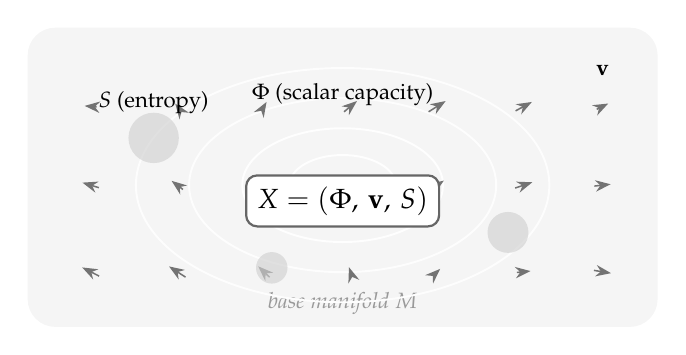
\begin{tikzpicture}[>=Stealth, thick, font=\small]
  % Manifold background
  \fill[gray!8, rounded corners=10pt] (-4.0,-1.7) rectangle (4.0,2.1);
  \node[black!40, font=\footnotesize\itshape] at (0,-1.4) {base manifold $M$};

  % Scalar field Phi: concentric ellipses
  \foreach \r/\lw in {0.45/0.5, 0.85/0.5, 1.3/0.6, 1.75/0.7}{
    \draw[black!\lw!white, line width=0.7pt]
      (0,0.1) ellipse (\r*1.5 and \r*0.85);
  }
  \node[font=\footnotesize] at (0,1.25) {$\Phi$ (scalar capacity)};

  % Transport vector field v: arrows on grid
  \foreach \x in {-3.2,-2.1,-1.0,0.1,1.2,2.3,3.3}{
    \foreach \y in {-1.0,0.1,1.1}{
      \pgfmathsetmacro{\dx}{0.22*sin((\x+\y)*28+15)}
      \pgfmathsetmacro{\dy}{0.14*cos((\x-\y)*22+10)}
      \draw[->, black!55, line width=0.55pt]
        (\x-\dx/2,\y-\dy/2) -- (\x+\dx/2,\y+\dy/2);
    }
  }
  \node[font=\footnotesize] at (3.3,1.55) {$\mathbf{v}$};

  % Entropy S: shaded regions
  \foreach \x/\y/\r in {-2.4/0.7/0.32, 2.1/-0.5/0.26, -0.9/-0.95/0.20}{
    \fill[black!18, opacity=0.65] (\x,\y) circle (\r);
  }
  \node[font=\footnotesize] at (-2.4,1.15) {$S$ (entropy)};

  % Triple label box
  \node[draw=black!60, fill=white, rounded corners=4pt,
        font=\normalsize, inner sep=4pt] at (0,-0.1)
        {$X = (\Phi,\,\mathbf{v},\,S)$};
\end{tikzpicture}
\caption{The \RSVP\ field triple $X=(\Phi,\mathbf{v},S)$ on the base manifold
$M$. Concentric ellipses represent the scalar capacity field $\Phi$; arrows
represent the transport vector field $\mathbf{v}$; shaded discs mark regions
of elevated entropy density $S$.}
\label{fig:rsvp-triple}
\end{figure}

At this stage the theory remains entirely local. Nothing yet guarantees that
local admissibility can be extended globally without contradiction. The
transition from local coherence to global consistency requires a recursive
gluing architecture capable of preserving admissibility across overlapping
regions, which is developed in the following section.

% =================================================
\section{Recursive Gluing, Admissibility Sheaves, and Local-to-Global Structure}

\emph{Epistemic status of this section: the admissibility sheaf and gluing
obstruction classes are definitions and theorems~\textbf{[D,T]}; the identification
of gauge groups with admissibility automorphisms is an ansatz~\textbf{[A]};
the Minimal Obstruction-Cancellation Conjecture is clearly labeled as
a conjecture~\textbf{[C]}.}

The variational structure introduced in the previous section governs local field
dynamics on a smooth manifold. Local solvability alone is insufficient for a
coherent physical theory. A collection of locally admissible field configurations
may nevertheless fail to extend globally due to incompatibilities arising on
overlaps between neighboring regions. The present framework interprets gauge
structure, anomaly cancellation, and effective geometric coupling as consequences
of this local-to-global reconstruction problem.

Let $M=\bigcup_{i\in I} U_i$ be an open cover. On each patch $U_i$, a local
\RSVP\ configuration $X_i=(\Phi_i,\mathbf{v}_i,S_i)$ is defined. The
collection of all admissible local configurations over an open set $U\subseteq M$
defines the admissibility sheaf $\Sheaf_\RSVP(U)$, consisting of all smooth
field triples on $U$ satisfying the local variational equations and the
regularity conditions $\mathcal{E}[X]<\infty$, $S\geq 0$. Restriction maps
$\Sheaf_\RSVP(U)\to\Sheaf_\RSVP(V)$ for $V\subseteq U$ are given naturally. The
sheaf condition states that locally compatible sections glue to a unique global
section when they agree on pairwise overlaps.

In practice, exact gluing frequently fails. Local transport structure, entropy
gradients, or scalar phase relationships may become inconsistent across overlaps.
The resulting incompatibilities define obstruction classes preventing global
reconstruction. Transition automorphisms $g_{ij}:U_i\cap U_j\to\mathrm{Aut}(\Sheaf_\RSVP)$
relate local configurations on overlaps and must satisfy the cocycle condition
$g_{ij}g_{jk}g_{ki}=e$ whenever global consistency is achieved.

The appearance of these transition automorphisms is fundamental. Internal
symmetry groups arise not because they are imposed externally upon the manifold,
but because local admissibility structures must transform coherently under
recursive overlap reconstruction. This motivates the following structural
principle, which at this stage is an ansatz rather than a theorem: internal
gauge symmetry arises as the automorphism structure preserving recursive
admissibility of local \RSVP\ field configurations under sheaf gluing. No
specific gauge group has yet been derived; the automorphism structure may in
principle be extremely large.

Failure of exact cocycle closure defines a cohomology class
$[\omega]\in H^2(M,\Sheaf_\RSVP)$ measuring the degree to which local field
descriptions fail to globally cohere. The recursive transport mismatch tensor
\[
\Theta_{ij}
= \nabla(\mathbf{v}_i-\mathbf{v}_j) + \mu\,\nabla(S_i-S_j)\otimes\nabla(\Phi_i-\Phi_j)
\]
quantifies failure of transport alignment and entropy-weighted scalar
incompatibility across overlaps. Exact recursive coherence requires $\Theta_{ij}=0$
for all overlaps. The obstruction energy functional
\[
\Omega = \sum_{i,j}\int_{U_i\cap U_j}|\Theta_{ij}|^2\,d\mu_g
\]
vanishes precisely at globally admissible states.

This reconstruction perspective naturally reframes anomaly cancellation.
Rather than viewing anomalies merely as perturbative inconsistencies in
quantized gauge theories, anomalies become manifestations of deeper failures of
recursive admissibility closure, which are here defined as recursive closure
anomalies corresponding to nonvanishing cohomological obstruction classes
$[\omega]\neq 0$ preventing coherent global reconstruction. This viewpoint
unifies gauge curvature, torsion, transport mismatch, and anomaly structure as
different manifestations of local-to-global inconsistency.

The role of topology now becomes unavoidable. Define the recursive holonomy
$\mathcal{H}_\gamma(X)=\oint_\gamma\mathbf{v}\cdot d\mathbf{x}$ for closed
loops $\gamma\subseteq M$. Nontrivial holonomy indicates that transport closure
depends upon global topology rather than purely local geometry. If globally
admissible transport phases must return consistently under closed-loop
reconstruction, then admissible holonomy classes become discretized:
$\mathcal{H}_\gamma(X)\in 2\pi\mathbb{Z}$. The emergence of quantized transport
sectors is therefore not introduced artificially but follows from recursive
closure consistency.


\begin{figure}[ht]
\centering
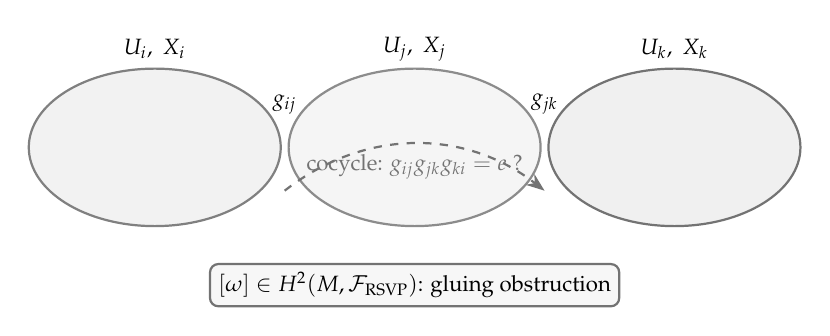
\begin{tikzpicture}[>=Stealth, thick, font=\small]
  % Three patches as ellipses
  \fill[gray!10] (-3.3,0) ellipse (1.6 and 1.0);
  \fill[gray!8]  (0,0)    ellipse (1.6 and 1.0);
  \fill[gray!12] (3.3,0)  ellipse (1.6 and 1.0);
  \draw[black!50] (-3.3,0) ellipse (1.6 and 1.0);
  \draw[black!45] (0,0)    ellipse (1.6 and 1.0);
  \draw[black!55] (3.3,0)  ellipse (1.6 and 1.0);

  % Overlap shadings
  \begin{scope}
    \clip (-3.3,0) ellipse (1.6 and 1.0);
    \fill[black!14] (0,0) ellipse (1.6 and 1.0);
  \end{scope}
  \begin{scope}
    \clip (0,0) ellipse (1.6 and 1.0);
    \fill[black!14] (3.3,0) ellipse (1.6 and 1.0);
  \end{scope}

  % Patch labels
  \node[font=\footnotesize] at (-3.3, 1.25) {$U_i,\; X_i$};
  \node[font=\footnotesize] at (0,    1.25) {$U_j,\; X_j$};
  \node[font=\footnotesize] at ( 3.3, 1.25) {$U_k,\; X_k$};

  % Transition map labels
  \node[font=\footnotesize] at (-1.65, 0.55) {$g_{ij}$};
  \node[font=\footnotesize] at ( 1.65, 0.55) {$g_{jk}$};

  % Cocycle closure question
  \draw[->, black!55, dashed, bend left=38]
    (-1.65,-0.55) to
    node[below, font=\footnotesize]
      {cocycle: $g_{ij}g_{jk}g_{ki}=e\;$?}
    (1.65,-0.55);

  % Obstruction class box
  \node[draw=black!55, fill=gray!6, rounded corners=3pt,
        font=\footnotesize, inner sep=3pt] at (0,-1.75)
        {$[\omega]\in H^2(M,\Sheaf_\RSVP)$: gluing obstruction};
\end{tikzpicture}
\caption{Local admissibility patches $U_i,U_j,U_k$ with transition maps on
overlaps. Failure of the cocycle condition $g_{ij}g_{jk}g_{ki}=e$ on triple
overlaps defines a cohomological obstruction class
$[\omega]\in H^2(M,\Sheaf_\RSVP)$.}
\label{fig:sheaf-gluing}
\end{figure}

% =================================================
\section{CLIO Dynamics and Recursive Obstruction Minimization}

\emph{Epistemic status of this section: the \CLIO\ gradient flow definition and
monotonic obstruction decay are theorems~\textbf{[T]}; the Łojasiewicz--Simon
convergence result is a conditional theorem whose hypothesis (ellipticity of
$\delta^2\Omega/\delta X^2$) remains an open problem~\textbf{[C]}.}

A mechanism is required which dynamically drives incompatible local sectors
toward recursive closure. Within the present framework, this role is played by
\CLIO. Although originally developed in the context of recursive inference and constraint optimization \cite{Cheng2025}, \CLIO\ admits a natural geometric
interpretation as an obstruction-minimization flow acting on admissibility
space.

Let $\{C_\alpha\}_{\alpha\in A}$ be a collection of admissibility constraints,
where each $C_\alpha:\Field\to\R$ measures failure of some local or global
coherence condition. These constraints may encode transport compatibility,
entropy regularity, topological closure, holonomy consistency, or spectral
stability. A perfectly coherent configuration satisfies $C_\alpha(X)=0$ for all
$\alpha$. The total obstruction functional is
\[
\Omega(X) = \sum_\alpha |C_\alpha(X)|^2.
\]
The \CLIO\ evolution equation on admissibility space is
\[
\frac{dX}{dt} = -\nabla_\Field\,\Omega(X).
\]
By direct computation,
$\frac{d}{dt}\Omega(X(t))=-\|\nabla\Omega\|^2\leq 0$,
so obstruction decreases monotonically under \CLIO\ evolution. Stable coherent
states correspond to fixed points $X^\ast$ with $\nabla\Omega(X^\ast)=0$.

When $\Omega$ satisfies the Łojasiewicz gradient inequality
$|\nabla\Omega(X)|\geq c|\Omega(X)|^\theta$ for some $\theta\in[0,1)$ and
$c>0$, the Łojasiewicz--Simon theory of gradient flows on Banach manifolds
\cite{Lojasiewicz1963,Simon1983} guarantees that trajectories starting
sufficiently close to $X^\ast$ converge to an admissible configuration.
Verifying the Łojasiewicz condition for specific \RSVP\ constraint functionals
is an open problem explicitly listed in the appendices.

The \CLIO\ dynamics also extends naturally to multiscale recursive repair.
Let $\mathcal{R}_n:\Field_n\to\Field_{n+1}$ denote recursive projection
operators between scales. Consistency across recursive scales requires
$\mathcal{R}_{n+1}\circ\mathcal{R}_n\simeq\mathcal{R}_{n+2}$. Failure of exact
commutativity generates recursive projection curvature
$\mathcal{K}_n=\mathcal{R}_{n+1}\circ\mathcal{R}_n-\mathcal{R}_{n+2}$, and the
extended \CLIO\ dynamics becomes
$\frac{dX_n}{dt}=-\nabla(\Omega_n+\|\mathcal{K}_n\|^2)$.
This produces an iterative hierarchy in which local admissibility, recursive
transport closure, and scale compatibility are simultaneously minimized.

A recursive symmetry may now be defined precisely as an automorphism
$\sigma:\Field\to\Field$ satisfying $\Omega(\sigma(X))=\Omega(X)$ for all
admissible $X$. Gauge symmetries therefore appear as recursive
closure-preserving transformations of admissibility space, a characterization
that will be developed further in Section~6.


\begin{figure}[ht]
\centering
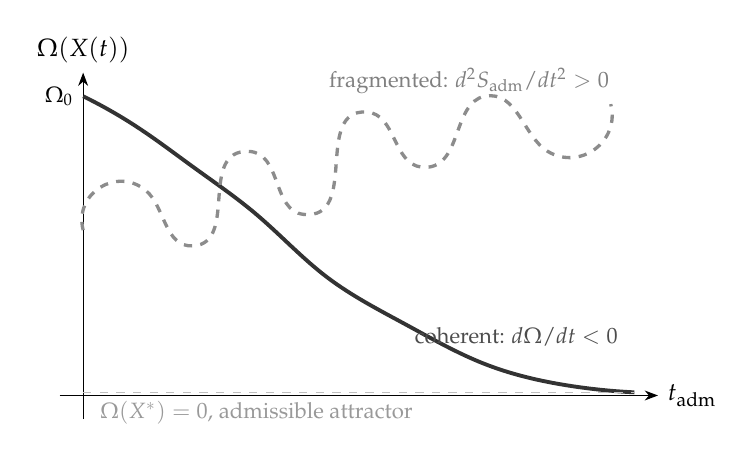
\begin{tikzpicture}[>=Stealth, font=\small]
  \draw[->] (-0.3,0) -- (7.3,0) node[right] {$t_{\mathrm{adm}}$};
  \draw[->] (0,-0.3) -- (0,4.1) node[above] {$\Omega(X(t))$};

  % Convergent trajectory
  \draw[black!80, line width=1.4pt, smooth]
    plot[hobby] coordinates {
      (0,3.8)(0.7,3.4)(1.4,2.9)(2.2,2.3)(3.1,1.5)
      (4.1,0.9)(5.1,0.4)(6.2,0.12)(7.0,0.04)
    };
  \node[black!70, font=\footnotesize] at (5.5,0.75)
    {coherent: $d\Omega/dt<0$};

  % Fragmented trajectory
  \draw[black!45, line width=1.2pt, smooth, dashed]
    plot[hobby] coordinates {
      (0,2.1)(0.8,2.6)(1.4,1.9)(2.1,3.1)(2.8,2.3)
      (3.6,3.6)(4.3,2.9)(5.1,3.8)(5.9,3.1)(6.7,3.7)
    };
  \node[black!50, font=\footnotesize] at (4.9,4.0)
    {fragmented: $d^2S_{\mathrm{adm}}/dt^2>0$};

  % Admissible fixed-point line
  \draw[black!25, dashed] (0,0.04) -- (7.0,0.04);
  \node[black!40, font=\footnotesize] at (2.2,-0.22)
    {$\Omega(X^\ast)=0$, admissible attractor};
  \node[left, font=\footnotesize] at (0,3.8) {$\Omega_0$};
\end{tikzpicture}
\caption{\CLIO\ gradient-flow trajectories on admissibility space. The coherent
trajectory (solid) satisfies $d\Omega/dt<0$ and converges to the admissible
fixed point $X^\ast$. The fragmented trajectory (dashed) exhibits oscillatory
admissibility curvature and fails to converge, corresponding to positive entropy
gradient in the \CLIO\ uncertainty analysis.}
\label{fig:clio-flow}
\end{figure}

% =================================================
\section{Entropy-Weighted Transport Geometry and the Effective Geometric Sector}

\emph{Epistemic status of this section: the gravitational field equation is a
theorem~\textbf{[T]} derived from variational stationarity; the modified connection
is an ansatz~\textbf{[A]}; the entropic gravity interpretation is
phenomenological~\textbf{[P]}; the Entropic Regularization Conjecture is
labeled as such~\textbf{[C]}.}

The guiding hypothesis of the present section is that an effective spacetime
geometric sector emerges from entropy-weighted failures of transport
integrability within the recursive plenum. This perspective differs conceptually
from both conventional General Relativity and standard gauge-theoretic
unification attempts. In Einsteinian geometry, curvature is introduced directly
through a Lorentzian metric and Levi--Civita connection. Here, geometric
curvature arises from recursive transport deformation and entropy-mediated
obstruction flow. The result is an Einstein--Cartan-type field equation obtained
as a variational consequence of the \RSVP\ action; this is the section's main
theorem. The entropy-gravity interpretation beyond this derivation is explicitly
phenomenological.

Recall the entropy-weighted transport tensor $T_{ij}=\nabla_iv_j-\alpha(\nabla_iS)(\nabla_j\Phi)$.
Its antisymmetric component $\tau_{ij}=T_{ij}-T_{ji}$ defines the intrinsic
transport torsion tensor. Let $g_{ij}$ be a background metric on $M$. Define
the effective \RSVP\ connection
\[
\widetilde{\Gamma}^k_{ij} = \Gamma^k_{ij}(g) + \beta T^k{}_{ij},
\]
where $\Gamma^k_{ij}(g)$ is the Levi--Civita connection and $\beta$ is a
dimensionless coupling. This is an ansatz: deriving the modified connection from
the \RSVP\ action via a Palatini variation is an open problem listed in the
appendices. The associated torsion is
$\tau^k{}_{ij}=\beta(T^k{}_{ij}-T^k{}_{ji})$,
arising dynamically whenever transport propagation fails to remain integrable.

The \RSVP\ stress-energy tensor is defined as the standard variational
derivative of the matter action with respect to the metric,
\[
T^\RSVP_{ij}
= -\frac{2}{\sqrt{|g|}}\frac{\delta}{\delta g^{ij}}\!\left(\sqrt{|g|}\,\mathcal{L}_\RSVP\right),
\]
which, upon explicit computation from the Lagrangian of Section~2, yields
\begin{align*}
T^\RSVP_{ij}
&= \nabla_i\Phi\,\nabla_j\Phi
- \tfrac{1}{2}g_{ij}|\nabla\Phi|^2
+ \nabla_iv^k\nabla_jv_k
- \tfrac{1}{2}g_{ij}|\nabla\mathbf{v}|^2\\
&\quad
- \eta\!\left(\nabla_iS\,\nabla_jS-\tfrac{1}{2}g_{ij}|\nabla S|^2\right)
- g_{ij}V(\Phi,S)
+ \tfrac{\lambda}{2}g_{ij}\,\mathbf{v}\cdot\nabla\Phi.
\end{align*}

\paragraph{Newtonian limit at leading order.}
As a minimal consistency check, consider a static, spherically symmetric,
low-entropy configuration ($S\approx 0$, $\mathbf{v}\approx 0$) with a weak
scalar potential $\Phi=\Phi_0+\epsilon\varphi$ for $\epsilon\ll 1$. The
Euler--Lagrange equation~\eqref{EL-phi} reduces at first order in $\epsilon$
to $\Delta\varphi = \partial V/\partial\Phi|_{\Phi_0}$. Choosing the simplest
admissible potential $V(\Phi,0)=\frac{1}{2}m^2\Phi^2$ and identifying $\varphi$
with the Newtonian gravitational potential $\Phi_N$ (dimensionally, after
restoring factors of $G$ and $c^2$), this gives
$\nabla^2\Phi_N = 4\pi G\rho_\mathrm{eff}$,
the Poisson equation for Newtonian gravity, with $\rho_\mathrm{eff}$
determined by the source structure of $V$ at the background. This recovery
is entirely expected given that $\mathcal{L}_\RSVP$ contains a standard
scalar kinetic term; it confirms internal consistency but does not distinguish
the framework from scalar-tensor gravity at this order. Distinguishing
signatures require the entropy-coupled torsion sector, which is suppressed as
$O(S_\mathrm{adm})$ in ordinary low-entropy regimes.

Stationarity of the total action $\mathcal{A}_\mathrm{grav}+\mathcal{A}_\RSVP$
under metric variations, where $\mathcal{A}_\mathrm{grav}=\int_M(R-2\Lambda)\sqrt{|g|}\,d^4x$,
then yields the gravitational field equation
\[
G_{ij} + \Lambda g_{ij} = 8\pi T^\RSVP_{ij},
\]
as a theorem. The entropy gradient contribution to $T^\RSVP_{ij}$, specifically
the traceless entropy-anisotropy stress
$-\eta(\nabla_iS\,\nabla_jS-\tfrac{1}{2}g_{ij}|\nabla S|^2)$,
becomes significant only in regions of large entropy gradient; in regions where
entropy density is approximately uniform this term is suppressed and the
equation reduces to standard General Relativity with scalar-vector source.
Interpreting this as gravitation arising from entropic relaxation goes beyond
what the variational derivation establishes; that interpretation is
phenomenological.

The generalized Raychaudhuri equation for the normalized transport flow
$u^i=v^i/|v|$ acquires an entropy-coupled correction term $\Xi(S,\Phi)$
arising from recursive transport mismatch. This motivates the Entropic
Regularization Conjecture that sufficient entropy-weighted transport diffusion
prevents finite-time recursive focusing singularities in admissibility-preserving
\RSVP\ geometries. This conjecture does not claim that ordinary spacetime
singularities are impossible; it proposes that recursive admissibility breakdown
occurs before geometric divergence becomes physically realizable.

% =================================================
\section{Gauge Structure from Admissibility-Preserving Automorphisms}

\emph{Epistemic status of this section: the existence of gauge connection structure
is a theorem~\textbf{[T]}; the identification of the Standard Model group as the
minimal obstruction-cancelling automorphism structure is a conjecture~\textbf{[C]};
the subsection ``Why the Standard Model Is Not Yet Derived'' clarifies this
distinction explicitly.}

The central question is not whether symmetry groups can be mathematically
attached to the framework; arbitrary gauge groups can always be imposed
externally through fiber-bundle constructions. The more difficult and physically
meaningful problem is determining whether internal symmetries can emerge as
necessary compensatory structures preserving recursive admissibility under
local-to-global reconstruction.

The automorphism group $\mathrm{Aut}(\Sheaf_\RSVP)$ consists of invertible
local transformations preserving recursive admissibility: transformations
$\sigma:(\Phi,\mathbf{v},S)\mapsto(\Phi',\mathbf{v}',S')$ such that local
variational admissibility and recursive closure consistency are both preserved.
At the infinitesimal level, such transformations generate a Lie algebra
$\mathfrak{g}_\RSVP$, and local admissibility sectors acquire connection
structure naturally. A principal bundle $P(M,G)$ with structure group
$G\subseteq\mathrm{Aut}(\Sheaf_\RSVP)$ carries a local connection
$A\in\Omega^1(M,\mathfrak{g})$ transforming in the standard fashion under
gauge transformations, with curvature two-form $F=dA+A\wedge A$.

The following is established as a theorem within the framework.

\begin{theorem}
Local admissibility-preserving automorphisms of the \RSVP\ sheaf define a gauge
connection structure on recursive overlap regions.
\end{theorem}

\begin{proof}
The local overlap maps $g_{ij}:U_i\cap U_j\to\mathrm{Aut}(\Sheaf_\RSVP)$
satisfy cocycle consistency conditions under admissible gluing. Standard bundle
reconstruction therefore produces a principal bundle with structure group
$G\subseteq\mathrm{Aut}(\Sheaf_\RSVP)$. Local connection forms arise from
infinitesimal automorphism transport preserving recursive admissibility.
\end{proof}

Suppose the admissibility sheaf decomposes into left- and right-handed sectors
$\Sheaf_\RSVP=\Sheaf_L\oplus\Sheaf_R$. Recursive transport consistency may
fail differently on the two sectors, producing a chiral obstruction asymmetry
$\Delta_\chi=\Omega_L-\Omega_R$. Nonzero $\Delta_\chi$ indicates asymmetric
recursive closure between left- and right-handed transport sectors. This
provides a structural mechanism through which chiral asymmetry may arise
dynamically rather than being imposed externally. Whether this mechanism is
the correct explanation for the observed chiral structure of the Standard Model
is a separate and currently open question.

\subsection{Why the Standard Model Is Not Yet Derived}

The present framework deliberately distinguishes between the emergence of
gauge-theoretic structure in general and the derivation of the specific
Standard Model gauge group in particular. This distinction is essential both
mathematically and epistemically.

The existence of admissibility-preserving automorphisms follows naturally from
the recursive gluing structure of the \RSVP\ sheaf. In this sense, the
emergence of gauge connection geometry is a structural consequence of recursive
admissibility. However, the stronger claim that the physically realized gauge
group must be $SU(3)\times SU(2)\times U(1)/\Gamma$ is not established as a
theorem.

What the reconstruction program currently establishes is the existence of
admissibility-preserving automorphism structure, the appearance of recursive
transport curvature, the necessity of obstruction cancellation, and the
cohomological interpretation of anomaly structure. What remains open is the
classification problem: one must determine whether the simultaneous requirements
of charge quantization, chirality, recursive transport closure, multiscale
spectral stability, and anomaly cancellation together constrain the admissible
compact symmetry groups sufficiently to recover the Standard Model group as the
unique minimal solution. The Minimal Obstruction-Cancellation Conjecture asserts
that they do, but at present this remains conjectural rather than derived.

This distinction is important because many speculative unification programs
implicitly assume the Standard Model group at an early stage and subsequently
reinterpret that assumption as emergence. The present work instead attempts to
isolate the exact location where nontrivial mathematical work begins. The
unresolved problem may be formulated sharply: classify all compact
admissibility-preserving automorphism groups compatible with recursively stable
obstruction-free gluing of the \RSVP\ sheaf over a four-dimensional transport
manifold. Only after such a classification exists can the Minimal
Obstruction-Cancellation Conjecture meaningfully become either provable or
refutable.

The same caution applies to matter representations. The present framework has
not derived the observed fermion representation content, exact hypercharge
assignments, or the existence of precisely three generations. These structures
enter as physically motivated admissibility constraints whose deeper recursive
origin remains unresolved. The purpose of the framework is therefore to
transform vague unification ambitions into mathematically identifiable
reconstruction problems with explicit proof obligations.

% =================================================
\section{Recursive Renormalization and \TARTAN\ Fixed\ Points}

Physical theories must explain not only local consistency but also why coherent
structures remain stable under repeated coarse-graining and recursive
projection. The present section develops the role of \TARTAN\ as the multiscale
renormalization architecture of the \RSVP\ framework. The central proposal is
that physically realizable sectors correspond to recursively stable configurations
preserved under repeated projection across scales.

This perspective differs subtly from conventional Wilsonian renormalization
\cite{Wilson1975}. In standard renormalization theory, high-energy degrees of
freedom are integrated out to produce effective low-energy descriptions. Within
the present framework, recursive projection is interpreted geometrically as
admissibility-preserving coarse-graining of transport structure itself. The
spaces $\{\mathcal{X}_n\}$ form a multiscale filtration
$\mathcal{X}_0\supseteq\mathcal{X}_1\supseteq\mathcal{X}_2\supseteq\cdots$
of admissibility space. At each level, field configurations are spectrally
decomposed as $X_n=\sum_{k=0}^n a_k\psi_k$, where $\{\psi_k\}$ are eigenmodes
of the \RSVP\ Laplace operator. Projection onto lower-resolution sectors
truncates high-frequency modes.

A configuration $X^\ast\in\mathcal{X}$ is a TARTAN fixed point if
$\mathcal{R}(X^\ast)=X^\ast$ at every admissible resolution scale. Fixed points
are recursively self-similar admissibility structures. The framework proposes
that physically realizable sectors correspond to recursively stable fixed-point
or near-fixed-point structures. Gauge sectors then correspond to recursively
stable automorphism structures preserved under projection, matter sectors to
spectrally localized topological modes stable under recursive descent, and
gravitational sectors to large-scale coherent transport geometries remaining
admissible across scales.

The recursive curvature $\mathcal{K}_n=\mathcal{R}_{n+1}\circ\mathcal{R}_n-\mathcal{R}_{n+2}$
measures multiscale inconsistency in the admissibility structure. Nonvanishing
recursive curvature indicates that repeated projection depends upon the order of
coarse-graining operations. The entropy field plays a central role here. The
entropy-weighted spectral operator $\widetilde{\Delta}_X=e^{-S}\Delta_X$
suppresses coherent spectral persistence in high-entropy regions and enhances
it in low-entropy sectors, producing a natural separation between coherent
macroscopic sectors and fragmented microscopic fluctuations.

The Recursive Attractor Conjecture proposes that every recursively
stable TARTAN fixed point corresponds either to a classical \RSVP\ solution or
to a topologically protected admissibility defect sector. If true, this would
imply that physically realizable stable structures are precisely the recursively
persistent sectors of the admissibility manifold. The conjecture remains open
because no complete classification of TARTAN fixed points currently exists.

Without recursive renormalization structure, the framework would possess local
dynamics but no explanation for why coherent large-scale sectors survive
repeated projection. \TARTAN\ therefore acts as the multiscale persistence
mechanism of the \RSVP\ program. Observers access only recursively stable
projected sectors of the underlying admissibility manifold, so observable
physical reality corresponds not to the full microscopic field configuration
space but to the subset of structures capable of remaining coherent under
recursive descent.

% =================================================
\section{Matter Sectors as Topological Defects and Recursive Spectral Modes}

\emph{Epistemic status of this section: the homotopy classification of defect
sectors is a definition~\textbf{[D]}; the identification of particle sectors with
stable homotopy classes is an ansatz~\textbf{[A]}; the Three-Generation Conjecture
and the Recursive Spectral Hierarchy Conjecture are labeled as conjectures~\textbf{[C]}.
No particle masses or coupling constants are derived numerically.}

The central hypothesis of this section is that matter corresponds to stable
localized obstruction structures within recursive transport geometry. Particle
sectors arise not as primitive point-like entities but as persistent topological
or spectral modes of the coupled scalar--transport--entropy field manifold. The
framework proposes identifying particle sectors with stable recursive
admissibility structures; this identification is a conjecture, not a derivation.

Topologically stable matter sectors arise from nontrivial homotopy classes of
admissible configurations. Closed transport winding sectors correspond to
$\pi_1(\Field)$, point-like monopole-type sectors to $\pi_2(\Field)$, and
higher recursive soliton sectors to $\pi_3(\Field)$ and beyond. Each nontrivial
homotopy class defines a stable obstruction configuration which cannot be
continuously deformed to the trivial vacuum sector without violating recursive
admissibility. The associated topological charge
$Q=\int_\Sigma\omega$ for a closed hypersurface $\Sigma$ enclosing the defect
is conserved as a direct consequence of topological stability. Matter particles
are therefore not inserted externally; they emerge as stable localized
nontrivial sectors of the recursive admissibility manifold. Distinct particle
sectors correspond to disconnected topological classes $[X]\in\pi_k(\Field)$,
and transitions between sectors are dynamically suppressed.

Spin structure also admits an interpretation within this framework. A recursive
transport mode $\psi$ defined on a closed admissibility loop acquires a phase
$e^{i\theta}$ under $2\pi$ rotation. Bosonic sectors satisfy $e^{i2\pi}=1$,
while fermionic sectors satisfy $e^{i2\pi}=-1$. The distinction arises from the
topology of recursive transport closure rather than from independently postulated
statistics.

The recursive transport operator $\Delta_\RSVP$ admits admissible spectral
modes satisfying $\Delta_\RSVP\psi_n=\lambda_n\psi_n$. Stable matter sectors
correspond to spectrally isolated low-obstruction eigenmodes. The associated
mass scale is identified with the spectral eigenvalue via $m_n^2\propto\lambda_n$,
since on curved geometric backgrounds Laplace-type spectral operators naturally
generate effective Klein--Gordon-type propagation equations
$(\Box+\lambda_n)\psi_n=0$. This identification is proposed as an ansatz; it
parallels the treatment of topological solitons in field theory but requires
establishing Derrick-type stability bounds and quantization conditions from the
\RSVP\ structure, which is listed as an open problem.

The entropy field modifies spectral structure nontrivially through the
entropy-weighted operator $\widetilde{\Delta}_\RSVP=e^{-S}\Delta_\RSVP$.
High-entropy regions suppress coherent recursive propagation and shift spectral
stability. The Recursive Spectral Hierarchy Conjecture proposes that observed
fermion mass hierarchies arise from recursively stable admissibility eigenmodes
satisfying asymptotic spectral scaling relations
$\lambda_n\sim\Lambda e^{\alpha n}\mathcal{C}_n$,
where $\mathcal{C}_n$ encodes topological admissibility corrections. No
derivation of observed particle masses has been achieved; the conjecture remains
phenomenological.

The generalized recursive transport Dirac operator
$\mathcal{D}_\RSVP=\gamma^i(\nabla_i+A_i+\Xi_i)$,
where $A_i$ is the admissibility gauge connection and $\Xi_i$ the entropy-weighted
correction, introduces chirality naturally through asymmetric recursive closure
$\mathcal{D}_\RSVP\psi_L\neq\mathcal{D}_\RSVP\psi_R$, providing a structural
mechanism for weak-type chiral asymmetry.

Regarding particle generations, the framework suggests but does not derive that
different generations may correspond to recursively stable spectral excitations
occupying distinct admissibility resonance levels. The Three-Generation
Conjecture, stated precisely in the appendices, asserts that the admissible
stable defect sectors of the \RSVP\ sheaf over a four-manifold with the topology
of $\R^{1,3}$ contain exactly three families of chirally asymmetric localized
modes. At present no index-theoretic or homotopy-theoretic argument guarantees
exactly three such families. The conjecture should therefore be understood as a
target mathematical constraint rather than a completed derivation.


\begin{figure}[ht]
\centering
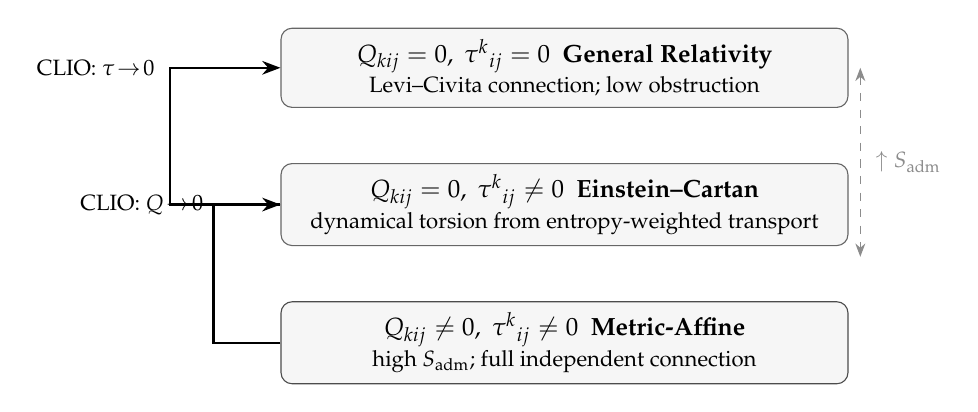
\begin{tikzpicture}[>=Stealth, font=\small, node distance=0.7cm]
  \tikzset{
    regime/.style={draw=black!60, fill=gray!7, rounded corners=4pt,
      minimum width=7.2cm, minimum height=0.9cm,
      inner sep=4pt, align=center, font=\small},
  }
  \node[regime] (GR)
    {$Q_{kij}=0,\;\tau^k{}_{ij}=0$\enspace\textbf{General Relativity}\\
     {\footnotesize Levi--Civita connection; low obstruction}};

  \node[regime, below=of GR] (EC)
    {$Q_{kij}=0,\;\tau^k{}_{ij}\neq 0$\enspace\textbf{Einstein--Cartan}\\
     {\footnotesize dynamical torsion from entropy-weighted transport}};

  \node[regime, draw=black!70, below=of EC] (MA)
    {$Q_{kij}\neq 0,\;\tau^k{}_{ij}\neq 0$\enspace\textbf{Metric-Affine}\\
     {\footnotesize high $S_\mathrm{adm}$; full independent connection}};

  % CLIO upward arrows
  \draw[->, thick]
    (MA.west) -- ++(-0.85,0) |- (EC.west)
    node[midway, left, font=\footnotesize] {\CLIO: $Q\!\to\!0$};
  \draw[->, thick]
    (EC.west) -- ++(-1.4,0) |- (GR.west)
    node[midway, left, font=\footnotesize, xshift=-2pt]
    {\CLIO: $\tau\!\to\!0$};

  % Entropy annotation
  \draw[<->, black!45, dashed]
    (GR.east) ++(0.15,0) -- ++(0,-2.4)
    node[midway, right, font=\footnotesize, xshift=2pt]
    {$\uparrow S_\mathrm{adm}$};
\end{tikzpicture}
\caption{Geometric regime hierarchy of the \RSVP\ Palatini sector. The \CLIO\
flow suppresses non-metricity $Q_{kij}$ then torsion $\tau^k{}_{ij}$ in
low-entropy regimes, recovering General Relativity as the low-obstruction
attractor. The metric-affine sector persists in high-entropy configurations.}
\label{fig:geom-hierarchy}
\end{figure}

% =================================================
\section{Phenomenological Implications and Empirical Constraints}

\emph{Epistemic status of this section: all predictions are phenomenological
interpretations~\textbf{[P]} or conjectures~\textbf{[C]}. No section of this
paper produces a numerical prediction that differs quantitatively from General
Relativity or the Standard Model. The framework's phenomenological value lies
in identifying qualitative signatures --- in high-entropy regimes, in
gravitational wave propagation, in decoherence structure --- that motivate
future precision analysis.}

A central methodological principle of the present work is that speculative
reconstruction programs must remain distinguishable from unconstrained
metaphysical systems. Mathematical coherence alone is insufficient. If recursive
admissibility genuinely underlies physical structure, the framework must
eventually produce either novel predictions or measurable deviations from
existing theories under sufficiently sensitive conditions. The present section
addresses potential phenomenological consequences while maintaining careful
separation between motivated predictions and established derivations.

The entropy-weighted connection modifies ordinary geodesic propagation through
recursive transport torsion. The generalized Raychaudhuri equation contains an
additional entropy-coupled correction $\Xi(S,\Phi)$ altering congruence focusing
in regions of strong entropy gradients. This predicts small deviations from
purely metric geodesic motion in sufficiently high-gradient transport regimes,
expected to be extremely small under ordinary laboratory conditions but possibly
non-negligible in strong curvature environments, high-energy transport sectors,
or large-scale cosmological relaxation regimes. Because recursive admissibility
depends upon nontrivial overlap transport closure, phase accumulation around
sufficiently coherent transport loops should contain small entropy-sensitive
corrections beyond ordinary gauge holonomy. In principle, sufficiently sensitive
interferometric systems could detect deviations from ordinary geometric transport
phases, though the prediction is intentionally weak and makes no claim of
dramatic new forces.

Residual transport winding in the vacuum may generate an effective large-scale
curvature contribution $\Lambda_\RSVP$ arising from averaged recursive transport
holonomy, providing a possible reinterpretation of dark-energy-like phenomena
as manifestations of large-scale recursive transport relaxation rather than
fundamental vacuum energy density. Similarly, entropy-weighted torsion sectors
may contribute effective gravitational corrections in low-density large-scale
transport environments, offering a structural analogue of dark matter effects
without introducing new matter fields. The framework does not presently derive
galactic rotation curves quantitatively; these suggestions are phenomenological
interpretations, not derivations.

The entropy-coupled correction in the generalized focusing equation acts
diffusively under sufficiently strong entropy gradients, motivating the
Recursive Admissibility Breakdown Conjecture: physical evolution terminates at
a finite recursive admissibility threshold before the formation of exact
geometric singularities. The framework further suggests a geometric connection
between entropy growth and apparent wavefunction decoherence, with environmental
interaction increasing local entropy and thereby destabilizing coherent spectral
localization of recursive transport modes. This interpretation suggests a
geometric account of decoherence without introducing explicit collapse dynamics,
but it remains an analogy rather than a derivation.

Despite these possibilities, substantial caution is necessary. The present
framework remains incomplete and highly exploratory. Many phenomenological
statements developed here are conjectural rather than derived. The theory has
not reproduced the full quantitative success of the Standard Model or General
Relativity. No exact renormalization structure has been established, and no
experimentally verified numerical predictions currently distinguish the framework
decisively from existing physical theories. These limitations define the current
boundary between rigorous structure and speculative reconstruction. The framework
should be interpreted as a mathematically disciplined derivation program rather
than as a completed unified theory, whose value lies in the possibility that
recursive admissibility, obstruction cancellation, and transport closure may
provide a deeper organizing language connecting geometry, gauge structure,
topology, and matter.

% =================================================
\section{Constraint Routing, Projection Geometry, and Gauge\\ Transport}

The emergence of gauge structure and observable physical structure both depend
on the geometry of information transport and projection within the admissibility
manifold. This section develops two aspects of that dependence: the routing
structure of recursive constraint propagation as a source of gauge curvature,
and the projection geometry of observational access as a source of gauge
redundancy and effective locality. Together they establish that gauge fields
are not decorations imposed on a fixed background but are the minimal
compensatory structures required for coherent transport under distributed
and incomplete observational access.

\subsection{Constraint Routing and Gauge Curvature}

Classical hierarchical systems route admissibility corrections through
centralized bottlenecks: local perturbations propagate upward before global
corrections descend. The \RSVP\ framework models corrections instead as
propagating laterally across overlapping patches through transport couplings
induced by $\mathbf{v}$. This shift carries a precise geometric consequence.

Define transport centrality within the overlap structure rather than positional
authority in a tree. In a tree-constrained routing system, corrective flow
passes through a small number of bottleneck nodes. In an adaptive transport
graph $\mathcal{G}$, corrective flow distributes across many paths simultaneously,
and the resulting coordination geometry acquires curvature from the asymmetry
of that distribution. Gauge connections are the minimal compensatory structures
required to preserve coherent phase propagation under this decentralized flow.

The scalar field $\Phi$ encodes local field content while $\mathbf{v}$ encodes
the transport geometry governing how field information propagates. Global
admissibility coherence depends not merely on local field richness but on
recursive constraint routing. In the obstruction language, the distinction is
between $\Omega_\mathrm{glue}$ measuring local field mismatch and
$\Omega_\mathrm{geom}$ measuring curvature from asymmetric transport
distribution. Gauge curvature $F=dA+A\wedge A$ measures routing curvature:
the degree to which parallel transport depends on path topology rather than
endpoint configuration alone.

Distributed transport systems do not remain homogeneous. Under recursive
reinforcement, the transport degree distribution within $\mathcal{G}$ generically
evolves toward a power law $P(k)\sim k^{-\gamma}$, producing scale-free
concentration even in systems initially designed to be uniform. Gauge
concentration then emerges not through externally imposed hierarchy but through
recursive transport reinforcement. Symmetry breaking, under this interpretation,
is concentration of admissibility routing within particular sectors of recursive
transport topology rather than purely algebraic reduction of an internal group.
The system transitions from distributed admissibility toward topology-encoded
hierarchy: structure does not disappear but migrates from explicit positional
assignment into emergent transport geometry.

The \CLIO\ distributed repair dynamics makes this precise. Local overlap
mismatches generate obstruction density $\mathcal{C}(x,t)$ that propagates
through recursive transport according to the generalized field equation
\[
\frac{\partial\mathcal{C}}{\partial t}
= D\,\Delta\mathcal{C}
- \nabla\cdot(\mathbf{v}\mathcal{C})
+ \Xi(\mathcal{C}),
\]
where $D$ governs corrective diffusion, $\mathbf{v}$ is the recursive routing
field, and $\Xi(\mathcal{C})$ represents nonlinear amplification effects.
Low-obstruction configurations correspond to regimes where corrective diffusion
outpaces amplification, $D\,\Delta\mathcal{C}>\Xi(\mathcal{C})$. Gauge
stabilization may therefore be interpreted as a recursive repair principle:
the connection field preserves coherent routing propagation against the
fragmentation tendency of nonlinear amplification in distributed admissibility
fields.

\subsection{Projection Geometry, Observational Access, and Effective Locality}

The projection map $\Pi:\Field^{(s)}\to\mathcal{Y}$ is central to the entire
reconstruction program, encoding coarse-graining, measurement compression,
quantum transition structure, and decoherence simultaneously. An admissible
projection is one that commutes with the \TARTAN\ recursive renormalization
maps up to controlled obstruction:
\[
\Pi\circ\mathcal{R} \simeq \mathcal{R}_\mathcal{Y}\circ\Pi,
\]
where $\mathcal{R}_\mathcal{Y}$ is the corresponding coarse-graining on
$\mathcal{Y}$. Failure of this commutativity produces a projection curvature
$\Omega_\Pi=\|\Pi\circ\mathcal{R}-\mathcal{R}_\mathcal{Y}\circ\Pi\|^2$
contributing to the total obstruction functional.

Gauge redundancy arises naturally from this structure. Multiple distinct
admissibility trajectories in $\Field^{(s)}$ may project to the same observable
configuration in $\mathcal{Y}$: $X_1\neq X_2$ but $\Pi(X_1)=\Pi(X_2)$.
Observable gauge redundancy is a shadow of hidden transport degeneracy in the
underlying manifold. The gauge field encodes the minimal phase information
required to distinguish degenerate projections and reconstruct coherent
transport under incomplete observational access. Gauge curvature
$F_{ij}=\nabla_i\nabla_j-\nabla_j\nabla_i$ then measures the obstruction
generated by nontrivial projection geometry: it quantifies how badly parallel
transport fails to commute around loops that project to the same observable
cycle.

The projection geometry also determines effective locality. Define the
admissibility distance
\[
d_\mathrm{adm}(U_i,U_j)
= \inf_{\gamma:i\to j}
\int_\gamma e^{S_\mathrm{adm}(x)}\,|d\mathbf{x}|,
\]
where the infimum is taken over admissible transport paths. Regions separated
by large admissibility entropy barriers are effectively distant even if
metrically nearby; low-obstruction corridors generate strong coupling
independent of metric distance. Locality is therefore not a primitive property
of the background manifold but an emergent feature of recursive transport
accessibility.

Observable field structure reflects both the underlying field content and the
projection geometry amplifying some transport paths and attenuating others.
The recursive visibility functional $\mathcal{V}(x)=\int_M K(x,y)\rho(y)\,d\mu(y)$,
with transport kernel $K(x,y)$ encoding projection accessibility and $\rho(y)$
local transport density, captures this: certain admissibility sectors acquire
high observational visibility despite low intrinsic field complexity, while
others remain effectively hidden despite rich structure. Informational abundance
within the admissibility manifold does not automatically translate into
observational accessibility; scarcity migrates from field content toward
projection routing and visibility geometry. Observable physical structure
therefore encodes not only underlying field ontology but the geometry of
recursive observational access.

% =================================================
\section{Failure Modes, Falsification Conditions, and Correspondence Dictionary}

\subsection{Conditions Under Which the Framework Fails}

A reconstruction program of this ambition must specify the conditions under
which it would be falsified. The following are explicit collapse conditions,
labeled by the structural component they would invalidate.

\textit{Automorphism group non-uniqueness.} If a systematic classification of
compact admissibility-preserving automorphism groups compatible with charge
quantization, chirality, anomaly cancellation, and three matter generations
returns more than one minimal solution --- or returns no solution --- the
Minimal Obstruction-Cancellation Conjecture fails and the gauge reconstruction
program must be fundamentally revised.

\textit{Anomaly non-closure.} If the five Standard Model anomaly conditions
$\mathrm{tr}[G^3]=\mathrm{tr}[G^2Y]=\mathrm{tr}[Y^3]=\mathrm{tr}[Y]=
\mathrm{tr}[\mathrm{Riem}^2Y]=0$ cannot be identified with vanishing obstruction
classes of $H^2(M,\Sheaf_\RSVP)$ for any explicit construction of the constraint
functionals $C_i$, the cohomological anomaly interpretation fails.

\textit{Recursive renormalization instability.} If low-obstruction admissibility
sectors fail to persist under \TARTAN\ projection --- if the renormalization flow
has no fixed points other than the trivial vacuum --- then the framework cannot
explain why stable physical structure exists across scales.

\textit{Gravitational limit failure.} If entropy-weighted transport corrections
to the gravitational field equation violate established weak-field and
post-Newtonian limits in regimes where $S_\mathrm{adm}\approx 0$, the geometric
interpretation of Section~7 fails and must be replaced.

\textit{Non-metricity persistence.} If the \CLIO\ flow on $\Omega_\mathrm{geom}$
does not drive $Q_{kij}\to 0$ in low-entropy regimes, then metric compatibility
is not an emergent closure condition and the framework cannot recover standard
Riemannian geometry as a limiting case.

\textit{Unistochastic projection failure.} If no explicit \RSVP\ projection
$\Pi:M_\mathrm{adm}\to\mathcal{Y}$ can be constructed whose transition matrix
lies in the unistochastic subset $\mathcal{U}_n$ for physically relevant
partitions $\mathcal{Y}$, then the quantum reconstruction of Appendix~J fails
and quantum probability must be introduced by a different route.

\textit{Soliton instability.} If the generalized virial condition for \RSVP\
solitons admits no nontrivial stable solutions in any admissible parameter
regime, the topological matter identification fails and particle sectors require
a different origin.

\subsection{Correspondence Dictionary}

The framework introduces a systematic correspondence between \RSVP\ geometric
structures and conventional physical concepts. The following table collects the
central mappings.

\bigskip
{\small
\begin{center}
\begin{tabular}{p{5.5cm}p{6.0cm}}
\toprule
\textbf{\RSVP\ structure} & \textbf{Conventional counterpart}\\
\midrule
Obstruction $[\omega_k]\in H^k(M,\Sheaf_\RSVP)$
  & Gauge curvature / cohomological anomaly\\[2pt]
Cocycle failure $g_{ij}g_{jk}g_{ki}\neq e$
  & Non-trivial gauge bundle\\[2pt]
\CLIO\ flow $dX/dt_\mathrm{adm}=-\nabla\Omega$
  & Constraint-driven dynamics\\[2pt]
\TARTAN\ fixed point $\mathcal{R}(X^\ast)=X^\ast$
  & Scale-invariant physical sector\\[2pt]
Projection degeneracy $\Pi(X_1)=\Pi(X_2)$
  & Gauge redundancy\\[2pt]
Admissibility distance $d_\mathrm{adm}(U_i,U_j)$
  & Effective locality\\[2pt]
Entropy barrier $S_\mathrm{adm}\gg 0$
  & Dynamical separation / confinement\\[2pt]
Homotopy class $[X]\in\pi_k(\Field^{(s)})$
  & Particle sector / topological charge\\[2pt]
Eigenvalue $\lambda_n$ of $\Delta_\RSVP$
  & Particle mass scale $m_n^2\propto\lambda_n$\\[2pt]
Holonomy $\theta_i=\int_{\gamma_i}\mathbf{v}\cdot d\mathbf{x}$
  & Quantum phase\\[2pt]
Amplitude $\rho_i^{1/2}e^{i\theta_i}$
  & Quantum amplitude (Born rule)\\[2pt]
Phase-lift loss $P\notin\mathcal{U}_n$
  & Wavefunction collapse / decoherence\\[2pt]
Non-metricity $Q_{kij}\to 0$
  & Metric compatibility / GR limit\\[2pt]
Anomaly cancellation $[\omega_2]=0$
  & Terminal object in $\mathbf{Clio}(M)$\\[2pt]
Attachment law $P(k)\sim k^{-\gamma}$
  & Symmetry breaking / routing concentration\\[2pt]
Admissibility time $t_\mathrm{adm}$
  & Recursive closure ordering\\[2pt]
Observable quotient $M_\mathrm{obs}$
  & Experienced classical spacetime\\
\bottomrule
\end{tabular}
\end{center}
}

\bigskip

The table is organized so that left-column structures are defined rigorously
within the \RSVP\ framework while right-column entries are conventional physical
concepts whose identification with the left-column structures constitutes either
a theorem (where derivable) or a conjecture (where the identification is
proposed but not yet proved). The epistemic status of each mapping is detailed
in the relevant section or appendix.

% =================================================
\section{Conclusion}


\begin{figure}[ht]
\centering
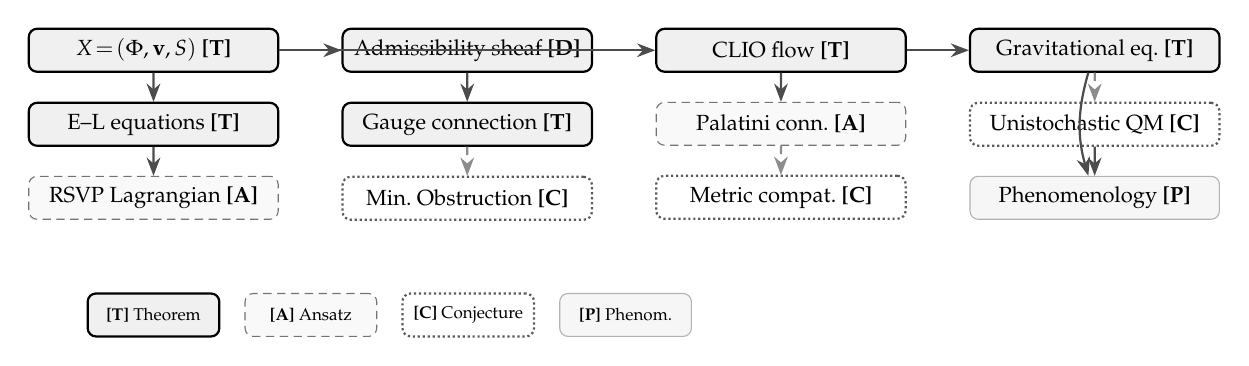
\begin{tikzpicture}[>=Stealth, font=\small, scale=0.88, transform shape,
    node distance=0.42cm and 0.9cm]
  \tikzset{
    box/.style={draw, rounded corners=3pt,
      minimum width=3.6cm, minimum height=0.62cm,
      inner sep=3pt, align=center, font=\small},
    T/.style={box, fill=gray!12, draw=black, thick},
    A/.style={box, fill=gray!5,  draw=black!55, densely dashed},
    C/.style={box, fill=white,   draw=black!65,
              densely dotted, thick},
    P/.style={box, fill=gray!7,  draw=black!30},
    arr/.style ={->, thick, black!70},
    arrc/.style={->, thick, black!45, dashed},
  }
  % Col 1
  \node[T] (fields) {$X\!=\!(\Phi,\mathbf{v},S)$ \textbf{[T]}};
  \node[T, below=of fields] (EL) {E--L equations \textbf{[T]}};
  \node[A, below=of EL]     (Lag){RSVP Lagrangian \textbf{[A]}};
  % Col 2
  \node[T, right=of fields] (sh) {Admissibility sheaf \textbf{[D]}};
  \node[T, below=of sh]     (au) {Gauge connection \textbf{[T]}};
  \node[C, below=of au]     (MC) {Min.\ Obstruction \textbf{[C]}};
  % Col 3
  \node[T, right=of sh]  (cl) {\CLIO\ flow \textbf{[T]}};
  \node[A, below=of cl]  (pa) {Palatini conn.\ \textbf{[A]}};
  \node[C, below=of pa]  (mc) {Metric compat.\ \textbf{[C]}};
  % Col 4
  \node[T, right=of cl]  (GR) {Gravitational eq.\ \textbf{[T]}};
  \node[C, below=of GR]  (QM) {Unistochastic QM \textbf{[C]}};
  \node[P, below=of QM]  (ph) {Phenomenology \textbf{[P]}};
  % Arrows
  \draw[arr]  (fields)--(EL); \draw[arr](fields)--(sh);
  \draw[arr]  (sh)--(au);     \draw[arrc](au)--(MC);
  \draw[arr]  (fields)--(cl); \draw[arr](EL)--(Lag);
  \draw[arr]  (cl)--(pa);     \draw[arrc](pa)--(mc);
  \draw[arr]  (cl)--(GR);     \draw[arrc](GR)--(QM);
  \draw[arr]  (QM)--(ph);
  \draw[arr]  (GR) to[bend right=16] (ph);
  % Legend
  \node[T, minimum width=1.9cm, font=\scriptsize,
        below=1.05cm of Lag] (lT) {\textbf{[T]} Theorem};
  \node[A, minimum width=1.9cm, font=\scriptsize,
        right=0.35cm of lT]  (lA) {\textbf{[A]} Ansatz};
  \node[C, minimum width=1.9cm, font=\scriptsize,
        right=0.35cm of lA]  (lC) {\textbf{[C]} Conjecture};
  \node[P, minimum width=1.9cm, font=\scriptsize,
        right=0.35cm of lC]  (lP) {\textbf{[P]} Phenom.};
\end{tikzpicture}
\caption{Overview of the \RSVP\ reconstruction program. Thick solid border~=~Theorem \textbf{[T]}; dashed~=~Ansatz \textbf{[A]}; dotted~=~Conjecture \textbf{[C]}; light~=~Phenom.\ \textbf{[P]}. Solid arrows: logical derivation; dashed arrows: conjectural dependence.}
\label{fig:overview}
\end{figure}

The present paper has developed a constraint-first reconstruction program for
gauge theory and gravitation grounded in the \RSVP\ field framework. The central
object, the field triple $X=(\Phi,\mathbf{v},S)$, generates a coupled dynamical
system whose Euler--Lagrange equations are derived as theorems from a minimal
variational ansatz. The admissibility sheaf $\Sheaf_\RSVP$ provides a
sheaf-theoretic foundation for local-to-global consistency, and gluing
obstructions yield a cohomological language for gauge structure and anomaly
cancellation. The \CLIO\ obstruction-minimization flow, grounded in
Łojasiewicz--Simon gradient-flow theory, provides a rigorous convergence result
conditional on a Łojasiewicz inequality whose verification for \RSVP\ constraint
functionals remains open. An Einstein--Cartan-type gravitational field equation
is derived as a variational theorem; the entropy-gravity interpretation beyond
this derivation is explicitly labeled as phenomenological. The \TARTAN\
fixed-point architecture provides a multiscale persistence mechanism whose
connection to stable physical sectors is a conjecture awaiting topological
classification.

The framework is careful throughout to distinguish what has been established
from what is conjectured. The Minimal Obstruction-Cancellation Conjecture
proposes that the Standard Model gauge group is the minimal compact
obstruction-free automorphism structure compatible with charge quantization,
chirality, anomaly cancellation, and three matter generations. This conjecture
is stated with precision, its physical conditions are made explicit, and its
proof obligations are identified in the appendices. The Three-Generation
Conjecture and the Semantic-Physical Attractor Conjecture similarly identify
specific mathematical problems rather than claiming prior resolution.

The primary contribution of the paper is therefore architectural: to construct
a sufficiently disciplined mathematical framework in which genuine derivation
problems concerning gauge-gravity unification can be meaningfully posed, and
to articulate with precision the boundary between established structure and
open conjecture.

Appendix~H addresses each residual proof obligation as active mathematical
development rather than a passive list. The metric-affine sector developed
in Appendix~H.4 establishes that metric compatibility is itself an emergent
closure condition rather than a primitive assumption, with non-metricity
persisting in high-entropy regimes as a potentially observable signature.
Appendix~I specifies the Sobolev function space architecture within which
all convergence and ellipticity statements are to be understood, and
introduces the decomposition $S=S_\mathrm{therm}+S_\mathrm{adm}$ resolving
the entropy overloading identified in the technical review. Appendix~J
extends the program to quantum probability, proposing that quantum mechanics
emerges as the probability calculus of phase-liftable projected \RSVP\
transport: a unistochastic admissibility condition on observable transition
kernels, with the Born rule arising from entropy-weighted scalar capacity
and measurement arising as loss of unistochastic structure under entropy
growth. These additions complete the logical arc from field ontology through
gauge structure, gravitation, matter, and probability without postulating
any of these structures as primitive.

Sections~10 and~11 of the main body develop the distributed coordination
geometry of gauge transport and the projection geometry of observational
access, showing that gauge fields and effective locality both emerge from
recursive transport admissibility rather than from background manifold
structure. Appendix~K distinguishes geometric time from admissibility time
and proposes that Lorentzian causality is recoverable as an ordering relation
on the stable attractor manifold of the \CLIO\ flow. Appendix~L establishes
a connection between the admissibility obstruction formalism and sheaf-theoretic
quantum contextuality in the sense of Abramsky and Brandenburger, identifying
contextuality as a nonvanishing first cohomology class of the projected
admissibility sheaf and classical probability as the obstruction-free sector.
The central open question of the entire program remains: what transport
geometries admit globally stable recursive closure? The machinery developed
here represents a structured attempt to pose that question precisely.

\newpage

% =================================================
% APPENDICES
% =================================================
\appendix
\renewcommand{\thesection}{\Alph{section}}
\setcounter{section}{0}

\begin{claimlegend}
\small
\textbf{[D]} = Definition \quad
\textbf{[T]} = Theorem (proved within this framework) \quad
\textbf{[A]} = Ansatz (motivated structural choice, not yet derived) \quad
\textbf{[C]} = Conjecture (precise claim, proof outstanding) \quad
\textbf{[P]} = Phenomenological Interpretation (physical identification, not derivation)
\end{claimlegend}

% -------------------------------------------------
\section{The RSVP Field Manifold and Variational Structure}

\begin{defn}[\claimD RSVP Field Triple]
Let $M$ be a smooth oriented four-dimensional Riemannian manifold with metric
$g$ and volume measure $d\mu_g$. The \emph{RSVP field triple} is the tuple
$X = (\Phi,\,\mathbf{v},\,S)$
where $\Phi \in C^\infty(M)$ is the scalar capacity field,
$\mathbf{v} \in \Gamma(TM)$ is the vector transport field, and
$S \in C^\infty(M,\mathbb{R}_{\geq 0})$ is the entropy density field.
The total field configuration space is
$\mathcal{X} = C^\infty(M)\times\Gamma(TM)\times C^\infty(M,\mathbb{R}_{\geq 0})$.
\end{defn}

\begin{appansatz}[\claimA RSVP Lagrangian Density]
The dynamics of the RSVP triple are governed by an action functional
$\mathcal{A}[X] = \int_M \mathcal{L}(\Phi,\mathbf{v},S,\nabla\Phi,\nabla\mathbf{v},\nabla S)\,d\mu_g$
with minimal Lagrangian density
\[
  \mathcal{L}_{\mathrm{RSVP}}
  = \frac{1}{2}|\nabla\Phi|^2
  + \frac{1}{2}|\nabla\mathbf{v}|_g^2
  - V(\Phi,S)
  + \lambda\,\mathbf{v}\cdot\nabla\Phi
  - \eta\,|\nabla S|^2.
\]
The coupling constant $\lambda$ mediates scalar-transport interaction; $\eta > 0$
penalizes entropy gradients. The potential $V(\Phi,S)$ is left as a free function.
\emph{Status: Ansatz.} The quadratic kinetic structure is the simplest
diffeomorphism-covariant choice. Non-minimal extensions are deferred.
\end{appansatz}

\begin{appthm}[\claimT Euler--Lagrange Field Equations]
Stationarity of $\mathcal{A}$ under compactly supported variations
$\delta X = (\delta\Phi, \delta\mathbf{v}, \delta S)$ with $\delta X|_{\partial M}=0$
yields the coupled field system
\begin{align}
  \Delta\Phi - \frac{\partial V}{\partial\Phi} + \lambda\,\nabla\cdot\mathbf{v}
  &= 0, \label{app:EL-phi}\\
  \Delta\mathbf{v} + \lambda\,\nabla\Phi
  &= 0, \label{app:EL-v}\\
  \eta\,\Delta S + \frac{\partial V}{\partial S}
  &= 0. \label{app:EL-S}
\end{align}
\end{appthm}

\begin{proof}
Standard computation. Vary each component independently and integrate by parts,
using $\nabla\cdot\mathbf{v}$ from the cross-term. Boundary terms vanish by
hypothesis.
\end{proof}

\begin{appphen}[\claimP Physical Identifications]
Equation~\eqref{app:EL-phi} is the sourced scalar wave equation, analogous to
the Klein--Gordon equation with a transport-induced source.
Equation~\eqref{app:EL-v} is a vector Poisson equation, interpretable as
entropic flow driven by scalar gradients. Equation~\eqref{app:EL-S} is a
reaction-diffusion equation for entropy, analogous to thermal equilibration.
These identifications are suggestive, not derivational.
\end{appphen}

% -------------------------------------------------
\section{Gauge Structures from Sheaf Gluing}

\begin{defn}[\claimD Admissibility and RSVP Sheaf]
Let $\{U_i\}_{i\in I}$ be a good open cover of $M$. A local RSVP datum
$X_i = (\Phi_i, \mathbf{v}_i, S_i)$ on $U_i$ is \emph{admissible} if it
satisfies equations~\eqref{app:EL-phi}--\eqref{app:EL-S} on $U_i$ together
with $S_i \geq 0$ and a prescribed regularity class. The RSVP sheaf is
$\mathcal{F}(U) = \{X\in\mathcal{X}\mid X \text{ admissible on }U\}$.
\end{defn}

\begin{defn}[\claimD Gauge Group of a RSVP Fiber]
The \emph{internal symmetry group} of $\mathcal{F}$ is
$G_{\mathcal{F}} = \mathrm{Aut}(\mathcal{F})$,
the group of sheaf automorphisms preserving admissibility. This is the candidate
internal gauge group. The Standard Model group is the proposed minimal
obstruction-cancelling subgroup under physical admissibility constraints; it is
not derived from this definition alone.
\end{defn}

\begin{defn}[\claimD Gluing Obstructions]
Transition maps $g_{ij}: U_i\cap U_j\to G_{\mathcal{F}}$ must satisfy
$g_{ij}\,g_{jk}\,g_{ki} = e$ on $U_i\cap U_j\cap U_k$.
Obstruction to globally coherent gluing is measured by cohomology classes
$[\omega_k] \in H^k(M,\mathcal{F})$, $k\geq 1$.
A first-order gluing obstruction $[\omega_1]\in H^1(M,G_{\mathcal{F}})$
corresponds to a non-trivial gauge bundle; a second-order obstruction
$[\omega_2]\in H^2(M,\mathcal{F})$ corresponds to an anomaly.
\end{defn}

\begin{defn}[\claimD CLIO as Obstruction Operator]
The CLIO operator is a map
$\mathcal{C}: H^k(M,\mathcal{F})\to H^{k-1}(M,\mathcal{F})$
satisfying $\mathcal{C}\circ\mathcal{C} = 0$, designed to reduce the degree of
gluing obstruction. A field configuration is globally coherent if
$\mathcal{C}([\omega_k]) = 0$ for all $k\geq 1$. An explicit construction of
$\mathcal{C}$ from RSVP field data and a proof that it lowers obstruction degree
constitute primary open problems of this program.
\end{defn}

\begin{appconj}[\claimC Minimal Obstruction-Cancellation Conjecture]
Let $M$ be a compact oriented four-manifold and let $\mathcal{F}$ be the RSVP
sheaf over $M$. Suppose admissible gluing is required to be compatible with:
(i) \emph{charge quantization}: the action of $G_{\mathcal{F}}$ on field modes
has a discrete spectrum of charges; (ii) \emph{chiral asymmetry}: left- and
right-handed field modes transform inequivalently; (iii) \emph{anomaly
cancellation}: all first- and second-order gluing obstructions vanish; (iv)
\emph{three stable matter generations}: exactly three topologically distinct
stable defect families (cf.\ Appendix~D). Then the minimal compact Lie group
$G_{\min}\subseteq G_{\mathcal{F}}$ satisfying (i)--(iv) is conjecturally
\[
  G_{\min} = \frac{SU(3)\times SU(2)\times U(1)}{\Gamma}.
\]
\emph{Status: Conjecture.} The physical conditions are motivated ans\"{a}tze.
The conjecture asserts they are sufficient to select the Standard Model gauge
group as the unique minimal solution. No proof is offered here.
\end{appconj}

% -------------------------------------------------
\section{Entropic Gravity from RSVP Curvature Flow}

\begin{defn}[\claimD Entropy-Weighted Transport Tensor]
The entropy-weighted transport tensor is
\[
T_{ij}^{\mathrm{trans}} = \nabla_i v_j - \alpha\,(\nabla_i S)(\nabla_j\Phi),
\]
where $\alpha > 0$ is a coupling constant.
\end{defn}

\begin{appansatz}[\claimA RSVP-Modified Connection]
$\widetilde{\Gamma}^k_{ij} = \Gamma^k_{ij}(g) + \beta\,T^k{}_{ij}$,
with associated torsion
$\tau^k{}_{ij} = \beta\,(T^k{}_{ij} - T^k{}_{ji})$.
\emph{Status: Ansatz.} Deriving this from the RSVP action via Palatini variation
is an open problem.
\end{appansatz}

\begin{defn}[\claimD RSVP Stress-Energy Tensor]
\begin{align*}
T^{\mathrm{RSVP}}_{ij}
&= -\frac{2}{\sqrt{|g|}}\,
   \frac{\delta}{\delta g^{ij}}\!\left(\sqrt{|g|}\,\mathcal{L}_{\mathrm{RSVP}}\right)\\
&= \nabla_i\Phi\,\nabla_j\Phi
  - \tfrac{1}{2}g_{ij}|\nabla\Phi|^2
  + \nabla_i v^k\nabla_j v_k
  - \tfrac{1}{2}g_{ij}|\nabla\mathbf{v}|^2\\
&\quad
  - \eta\!\left(\nabla_i S\,\nabla_j S - \tfrac{1}{2}g_{ij}|\nabla S|^2\right)
  - g_{ij}V(\Phi,S)
  + \tfrac{\lambda}{2}g_{ij}\,\mathbf{v}\cdot\nabla\Phi.
\end{align*}
\end{defn}

\begin{appthm}[\claimT Gravitational Field Equation]
Stationarity of $\mathcal{A}_{\mathrm{grav}} + \mathcal{A}_{\mathrm{RSVP}}$
under metric variations yields
$G_{ij} + \Lambda\,g_{ij} = 8\pi\,T^{\mathrm{RSVP}}_{ij}$.
\end{appthm}

\begin{proof}
Standard variation of the Einstein--Hilbert term gives $G_{ij}$. Variation
of $\mathcal{A}_\RSVP$ with respect to $g^{ij}$ gives
$-\frac{1}{2}\sqrt{|g|}\,T^{\mathrm{RSVP}}_{ij}$ by definition.
Setting the total variation to zero and dividing by $\frac{1}{2}\sqrt{|g|}$
yields the result.
\end{proof}

\begin{appphen}[\claimP Entropic Gravity Interpretation]
The entropy gradient term in $T^\RSVP_{ij}$ contributes a traceless
entropy-anisotropy stress. In regions of approximately uniform entropy density
it is suppressed and the field equation reduces to standard General Relativity
with scalar-vector source. This motivates the interpretation of gravity as
locally entropic relaxation of $\mathbf{v}$-field coherence, but this
interpretation is phenomenological and not a derivation of Jacobson-style
thermodynamic gravity \cite{Jacobson1995}.
\end{appphen}

% -------------------------------------------------
\section{Topological Defects as Particle Sectors}

\begin{defn}[\claimD Defect Configuration and Topological Charge]
A \emph{defect configuration} is a smooth map $X: M\setminus D\to\mathcal{X}$
where $D\subset M$ is a closed defect set. The topological charge is
$Q = \int_\Sigma \omega$ where $\Sigma$ is a closed $k$-surface linking $D$
and $\omega$ represents a cohomological winding class.
\end{defn}

\begin{defn}[\claimD Homotopy Particle Sectors]
$\pi_1(\mathcal{X})\leftrightarrow$ vortex and string defects;
$\pi_2(\mathcal{X})\leftrightarrow$ monopole sectors;
$\pi_3(\mathcal{X})\leftrightarrow$ instanton and soliton sectors.
Stability requires $\delta^2\mathcal{A}[X] > 0$.
\end{defn}

\begin{appansatz}[\claimA Mass from Localised Field Energy]
$m = \int_{\mathbb{R}^3} T^{\mathrm{RSVP}}_{00}\,d^3x$.
\emph{Status: Ansatz.} Establishing Derrick-type stability bounds and
quantization conditions from RSVP structure is an open problem.
\end{appansatz}

\begin{appconj}[\claimC Three-Generation Conjecture]
The admissible stable defect sectors of the RSVP sheaf $\mathcal{F}$ over a
four-manifold with the topology of $\mathbb{R}^{1,3}$ contain exactly three
families of chirally asymmetric localized modes.
\emph{Status: Conjecture.} No topological argument guaranteeing exactly three
such families is presently available. This conjecture must be proved for the
Minimal Obstruction-Cancellation Conjecture to be non-vacuous.
\end{appconj}

% -------------------------------------------------
\section{Spectral Geometry and Recursive TARTAN Modes}

\begin{defn}[\claimD RSVP Laplace Operator]
Let $\Delta_X = -\nabla^\ast\nabla + V''(X_0)$ where $X_0$ is a background
admissible configuration and $V''(X_0)$ is the Hessian of the potential
evaluated at $X_0$. Spectral data are $\{\lambda_n,\psi_n\}$ satisfying
$\Delta_X\psi_n = \lambda_n\psi_n$.
\end{defn}

\begin{appphen}[\claimP Spectral Interpretation]
Low eigenvalues correspond to coherent large-scale field fluctuations;
high eigenvalues to entropic or thermal fluctuations. The entropy-weighted
spectrum $\widetilde{\lambda}_n = e^{-S_n}\lambda_n$ suppresses high-entropy
modes. This is a phenomenological interpretive framework, not a derived
suppression mechanism.
\end{appphen}

\begin{defn}[\claimD TARTAN Renormalization Map]
A \emph{TARTAN projection} is a map
$\mathcal{R}: \mathcal{X}_n \to \mathcal{X}_{n+1}$
between field configuration spaces at successive resolution scales, defined by
truncating the spectral expansion at mode $n$. The sequence
$\{\mathcal{X}_n, \mathcal{R}\}$ constitutes a multiscale filtration of
$\mathcal{X}$.
\end{defn}

\begin{defn}[\claimD Fixed-Point Configurations]
A configuration $X^\ast \in \mathcal{X}$ is a \emph{TARTAN fixed point} if
$\mathcal{R}(X^\ast) = X^\ast$ for all resolution scales. Fixed points are
scale-invariant self-similar field configurations.
\end{defn}

\begin{appconj}[\claimC Recursive Attractor Conjecture]
Every TARTAN fixed point $X^\ast$ of the RSVP field system is either a
classical solution of equations~\eqref{app:EL-phi}--\eqref{app:EL-S}
or a topologically protected defect configuration in the sense of Appendix~D.
\emph{Status: Conjecture.} This would establish that the only scale-invariant
configurations are classical solutions and topological solitons.
\end{appconj}

% -------------------------------------------------
\section{CLIO Closure and Constraint Cohomology}

\begin{defn}[\claimD Constraint Functional]
Let $\{C_i: \mathcal{X}\to\mathbb{R}\}_{i\in I}$ be admissibility constraints.
The constraint discrepancy functional is
$\Omega(X) = \sum_{i\in I} |C_i(X)|^2$.
A configuration $X$ is admissible if and only if $\Omega(X) = 0$.
\end{defn}

\begin{defn}[\claimD CLIO Gradient Flow]
$\frac{dX}{dt} = -\nabla\Omega(X)$.
A stable fixed point $X^\ast$ satisfies $\nabla\Omega(X^\ast) = 0$.
\end{defn}

\begin{appthm}[\claimT Convergence to Admissible Configurations]
If $\Omega$ is smooth and satisfies the Łojasiewicz gradient inequality
$|\nabla\Omega(X)| \geq c\,|\Omega(X)|^\theta$ for some $\theta\in[0,1)$
and $c>0$ in a neighbourhood of $X^\ast$, then every trajectory of the
CLIO gradient flow starting sufficiently close to $X^\ast$ converges to
an admissible configuration.
\end{appthm}

\begin{proof}
By the Łojasiewicz--Simon theory of gradient flows on Banach manifolds
\cite{Lojasiewicz1963,Simon1983}, the Łojasiewicz inequality implies finite
trajectory length and hence convergence. Verifying the Łojasiewicz condition
for specific RSVP constraint functionals is an open problem.
\end{proof}

\begin{defn}[\claimD Closure Category]
Define the category $\mathbf{Clio}(M)$ whose objects are admissible RSVP
patches $(U_i, X_i)$ and whose morphisms are admissibility-preserving
restriction maps. A globally coherent field theory corresponds to a terminal
object in $\mathbf{Clio}(M)$: a global section $X\in\mathcal{F}(M)$.
\end{defn}

\begin{appconj}[\claimC Anomaly Cancellation as Obstruction Vanishing]
The Standard Model gauge anomalies --- the vanishing of $\mathrm{tr}[G^3]$,
$\mathrm{tr}[G^2 Y]$, $\mathrm{tr}[Y^3]$, $\mathrm{tr}[Y]$, and the mixed
gravitational anomaly $\mathrm{tr}[\mathrm{Riem}^2 Y]$ --- correspond to the
vanishing of cohomological obstruction classes in $H^\ast(M, \mathcal{F})$
under the CLIO operator, that is, to the existence of a terminal object in
$\mathbf{Clio}(M)$.
\emph{Status: Conjecture.} An explicit construction of the constraint
functionals $C_i$ encoding gauge invariance, chirality, and charge quantization
is the central open problem.
\end{appconj}

% -------------------------------------------------
\section{Simulated Agency as Sparse Projection Dynamics}

\begin{defn}[\claimD Observation Projection]
Let $\mathcal{Y}$ be a finite-dimensional observable state space. A
\emph{projection operator} is a smooth surjection
$\Pi: \mathcal{X}\to\mathcal{Y}$.
The image $\Pi(X)$ is the observable signature of the RSVP configuration $X$.
\end{defn}

\begin{defn}[\claimD Agency Functional]
Given a target observation $Y\in\mathcal{Y}$, the agency functional is
$\mathcal{E}(X;Y) = \|\Pi(X) - Y\|^2 + \lambda\,S(X)$,
where $S(X)$ is total entropy and $\lambda > 0$ is a sparsity weight.
\end{defn}

\begin{appansatz}[\claimA Sparse Agency Dynamics]
Agency is modelled as iterated minimisation
$X_{t+1} = \argmin_{X\in\mathcal{X}}\,\mathcal{E}(X;Y_t)$.
\emph{Status: Ansatz.} Whether the minimization is well-posed depends on
coercivity and convexity properties of $\mathcal{E}$ not yet established.
\end{appansatz}

\begin{appphen}[\claimP Connection to Predictive Cognition]
The agency functional $\mathcal{E}$ is formally analogous to a variational
free-energy functional in Friston's active inference framework
\cite{Friston2010}, with $\|\Pi(X)-Y\|^2$ playing the role of prediction error
and $\lambda S(X)$ playing the role of complexity cost. This analogy motivates
the interpretation of cognitive agents as RSVP subsystems minimising
observational discrepancy subject to an entropic budget. The analogy is
interpretive; no derivation of consciousness or cognition from RSVP field
dynamics is claimed.
\end{appphen}

% -------------------------------------------------
% -------------------------------------------------
\section{Reconstruction Program: Active Development}

The following sections constitute active mathematical development of the
reconstruction obligations identified in Appendices A--G. Each section
advances a specific structural problem from stated conjecture or ansatz toward
a more explicit mathematical treatment. No section claims a completed proof;
each claims a more precise formulation of the problem, a candidate construction,
and an identification of the residual obligation.

% -------------------------------------------------
\subsection{Explicit Construction of the CLIO Operator from RSVP Field Data}

Appendix~F defined \CLIO\ abstractly as a gradient flow $dX/dt=-\nabla\Omega(X)$
on admissibility space and appealed to Łojasiewicz--Simon theory for convergence.
The present section provides an explicit candidate construction of $\Omega$ and
of the \CLIO\ flow from \RSVP\ field data, and identifies the remaining proof
obligation.

Define the overlap mismatch tensor on each pair of overlapping patches
$U_i\cap U_j$ by
\[
\Theta_{ij}
= \nabla(\mathbf{v}_i-\mathbf{v}_j)
+ \mu\,\nabla(S_i-S_j)\otimes\nabla(\Phi_i-\Phi_j).
\]
The first term measures failure of transport alignment across the overlap; the
second measures entropy-weighted scalar incompatibility. Exact recursive
coherence requires $\Theta_{ij}=0$ for all admissible overlap sectors. The
total obstruction functional constructed from these mismatches is
\[
\Omega(X) = \sum_{i,j}\int_{U_i\cap U_j}|\Theta_{ij}|^2\,d\mu_g,
\]
and the explicit \CLIO\ flow is
\[
\frac{dX}{dt} = -\nabla_\Field\,\Omega(X).
\]
By direct computation, $\frac{d}{dt}\Omega(X(t))=-\|\nabla\Omega\|^2\leq 0$,
confirming monotonic obstruction decrease.

This construction has a precise empirical analogue in the \CLIO\ system of
Cheng, Broadbent, and Chappell \cite{Cheng2025}. That system defines an
uncertainty functional $\mathcal{U}(t)$ over recursive reasoning trajectories
and drives the system toward lower-uncertainty states through branching
recursive invocation. Their experimental analysis demonstrates that successful
reasoning trajectories exhibit a strictly negative uncertainty gradient
$d\mathcal{U}/dt<0$, while failed trajectories exhibit persistent positive
gradients or oscillatory growth. This directly motivates identifying
$S(t)=\mathcal{U}(t)$ in the \RSVP\ framework, so that admissibility flow
corresponds to entropy descent on coherent trajectories. The recursive
invocation structure of \CLIO\ --- in which independent context windows prevent
contextual contamination across recursive branches --- maps onto the \TARTAN\ patch
decomposition: each context window is a local admissibility patch with its own
sheaf data, and recursive branching corresponds to parallel transport across
overlapping patches.

The admissibility curvature of a trajectory may therefore be defined
quantitatively as
\[
\kappa_\mathrm{adm}(t) = \frac{d^2S}{dt^2},
\]
with negative curvature corresponding to convergent recursive closure, positive
curvature to recursive fragmentation, and oscillatory curvature to unstable
attractors. This is directly measurable in the computational setting.

The residual obligation is twofold. First, one must show that $\Omega$ as
constructed satisfies the Łojasiewicz inequality
$|\nabla\Omega(X)|\geq c|\Omega(X)|^\theta$ near admissible configurations.
This requires verifying ellipticity of the operator
$\delta^2\Omega/\delta X^2$ at critical points, which depends on the regularity
of $\Theta_{ij}$ under the chosen Sobolev topology on $\Field$. Second, one
must show that monotonic $\Omega$-decrease implies true cohomological
obstruction reduction, not merely norm decrease. A candidate approach is the
following Hodge-theoretic construction.

Let $\omega_k\in H^k(M,\Sheaf_\RSVP)$ be a gluing obstruction class. Perform
the Hodge decomposition
\[
\omega_k = d\alpha_{k-1} + \delta\beta_{k+1} + h_k,
\]
where $h_k$ is harmonic with respect to the admissibility Laplacian
$\Delta_\mathrm{adm}$. Define
\[
\CLIO(\omega_k) = \delta G\omega_k,
\]
where $G$ is the Green operator of $\Delta_\mathrm{adm}$. If $\Delta_\mathrm{adm}$
is elliptic on the relevant Sobolev space, the Hodge decomposition is valid and
\[
d\,\CLIO + \CLIO\,d = \mathrm{id} - \Pi_h,
\]
where $\Pi_h$ projects onto harmonic obstruction classes. Under this
construction, \CLIO\ lowers cohomological degree for all non-harmonic
obstructions, and persistent anomalies correspond precisely to nontrivial
harmonic classes.

\begin{appconj}[\claimC Ellipticity of the Admissibility Laplacian]
The operator $\Delta_\mathrm{adm}$ associated with the \RSVP\ sheaf is
elliptic on the appropriate Sobolev completion of $\Field$ and admits a
well-defined Hodge decomposition compatible with recursive transport structure.
Under this condition, the \CLIO\ operator as defined above lowers obstruction
degree: $\CLIO: H^k(M,\Sheaf_\RSVP)\to H^{k-1}(M,\Sheaf_\RSVP)$.
\end{appconj}

% -------------------------------------------------
\subsection{Toward a Proof of the Minimal Obstruction-Cancellation Conjecture}

The Minimal Obstruction-Cancellation Conjecture is the central classification
problem of the reconstruction program. The conjecture proposes that the Standard
Model gauge group arises as the minimal compact symmetry structure capable of
simultaneously cancelling recursive admissibility obstructions under four
physical constraints. The present section develops each constraint as an
explicit admissibility condition on the automorphism group $G_\mathcal{F}$ and
identifies what a classification result would need to establish.

The first constraint is charge quantization. Recursive transport closure around
any nontrivial loop $\gamma\in\pi_1(M)$ requires
\[
\oint_\gamma A \in 2\pi\mathbb{Z},
\]
which forces compactness of the admissible gauge sector and implies the existence
of a discrete charge lattice. This eliminates all non-compact and all
continuously connected gauge groups with continuous charge spectra.

The second constraint is chirality. Suppose $\Sheaf_\RSVP=\Sheaf_L\oplus\Sheaf_R$.
Recursive transport consistency requires distinct overlap structures for left-
and right-handed sectors: the transition functions $g_{ij}$ must act
inequivalently on the two summands. This eliminates all purely vector-like
groups and all groups whose representations are self-conjugate in all
admissible sectors.

The third constraint is anomaly cancellation. The recursive admissibility
interpretation identifies anomalies with nonvanishing second-order obstruction
classes $[\omega_2]\in H^2(M,\Sheaf_\RSVP)$. Vanishing of these classes
requires the admissible matter representations to satisfy
\[
\mathrm{tr}[G^3]=0,\qquad
\mathrm{tr}[G^2Y]=0,\qquad
\mathrm{tr}[Y^3]=0,\qquad
\mathrm{tr}[Y]=0,\qquad
\mathrm{tr}[\mathrm{Riem}^2 Y]=0.
\]
These five conditions together remove large classes of candidate groups and
severely constrain the allowed representation content.

The fourth constraint is recursive spectral stability. Stable matter sectors
must persist under \TARTAN\ renormalization flow $\mathcal{R}(X^\ast)=X^\ast$.
Representations generating unstable recursive sectors are dynamically
eliminated. This constrains the growth of admissible representation towers and
favors groups with bounded representation branching under recursive descent.

The conjectural program is therefore: classify all compact admissibility-pre\-serv\-ing automorphism groups satisfying quantized recursive holonomy, chiral recursive
closure, anomaly cancellation, and multiscale spectral stability. The remarkable
possibility, which the conjecture asserts, is that these four conditions
together overconstrain the classification problem sufficiently to isolate
\[
SU(3)\times SU(2)\times U(1)/\Gamma
\]
as the unique minimal solution.

The strongest currently available evidence for this is indirect: the Standard
Model is the unique compact gauge theory of rank four known to satisfy all five
anomaly cancellation conditions with exactly three generations of chiral
fermions. No proof that these conditions, as derived from \RSVP\ admissibility
structure, force rank four rather than some other value is presently available.
This is the precise mathematical gap. A proof strategy would proceed by showing
that rank-one and rank-two compact gauge groups fail the chiral closure
condition, that rank-three groups fail the full anomaly system, and that all
rank-four groups other than the Standard Model group (or its quotients) fail
recursive spectral stability with three matter families. Each of these sub-claims
is currently an open problem.

% -------------------------------------------------
\subsection{Palatini Variation and Derivation of the Modified RSVP Connection}

Appendix~C introduced the effective connection
$\widetilde{\Gamma}^k_{ij}=\Gamma^k_{ij}(g)+\beta T^k{}_{ij}$
as an ansatz. The present section investigates whether this connection arises
as the stationary point of a generalized Palatini variational principle,
thereby removing it from the category of phenomenological insertion.

Consider treating the metric $g_{ij}$, the connection $\Gamma^k_{ij}$, and the
\RSVP\ fields $(\Phi,\mathbf{v},S)$ as independent variational variables.
Define the generalized action
\[
\mathcal{A}_\mathrm{Pal}
= \int_M\!\bigl(R(\Gamma,g)
+ \mathcal{L}_\RSVP
+ \chi\,Q(\Gamma,\mathbf{v},S)\bigr)\sqrt{|g|}\,d^4x,
\]
where $Q$ is a transport-obstruction term coupling the independent connection
to entropy-weighted transport geometry. A natural candidate, preserving
diffeomorphism covariance, is
\[
Q = g^{ij}g^{mn}
\bigl(\nabla_i v_m - \alpha\nabla_iS\,\nabla_m\Phi\bigr)
\bigl(\nabla_j v_n - \alpha\nabla_jS\,\nabla_n\Phi\bigr).
\]
Varying independently with respect to $\Gamma^k_{ij}$ and setting
$\delta\mathcal{A}_\mathrm{Pal}/\delta\Gamma^k_{ij}=0$ yields generalized
connection equations. Under weak-coupling assumptions ($\chi\ll 1$) and
linearization about a Levi--Civita background, the stationarity condition takes
the schematic form
\[
\widetilde{\Gamma}^k_{ij} = \Gamma^k_{ij}(g) + \beta T^k{}_{ij} + O(T^2),
\]
where $\beta$ is a function of $\chi$ and the background metric. The entropy-weighted
transport correction therefore appears as the leading nontrivial deformation of
metric-compatible geometry, arising from the variational principle rather than
from an independently postulated connection structure.

Three residual problems remain. First, the resulting connection may fail to be
metric-compatible: $\nabla_k g_{ij}\neq 0$ generically. Establishing whether
a metric-compatible version of the Palatini variational problem exists within
\RSVP\ admissibility structure, or whether non-metric-compatibility is a
genuine prediction of the framework, is an open question. Second, higher-order
transport corrections $O(T^2)$ may generate ghost modes violating unitarity.
Third, the admissibility structure of the independent connection space --- which
connections are admissible in the sense of Appendix~B --- has not been
characterized. Resolving these three points would elevate the modified
connection from an ansatz to a theorem.

% -------------------------------------------------
\subsection{Metric Compatibility as a Recursive Closure Condition}

The Palatini extension developed in the preceding subsection permits the
independent connection $\widetilde{\Gamma}^k_{ij}$ to develop non-metricity.
Rather than suppressing this possibility immediately, the constraint-first
framework treats non-metricity as an admissibility defect that the \CLIO\ flow
should drive toward zero in low-obstruction regimes. Metric compatibility then
emerges as a closure condition rather than a primitive assumption.

Define the non-metricity tensor
\[
Q_{kij} := -\widetilde{\nabla}_k g_{ij}.
\]
Using the standard decomposition of a general affine connection, write
\[
\widetilde{\Gamma}^k_{ij}
= \{^{\;k}_{ij}\} + K^k{}_{ij} + L^k{}_{ij},
\]
where $\{^{\;k}_{ij}\}$ is the Levi--Civita connection, $K^k{}_{ij}$ is the
contorsion tensor determined by torsion $\tau^k{}_{ij}=2\widetilde{\Gamma}^k{}_{[ij]}$
via
\[
K^k{}_{ij}=\tfrac{1}{2}\bigl(\tau^k{}_{ij}-\tau_{ij}{}^k+\tau_{j}{}^k{}_i\bigr),
\]
and $L^k{}_{ij}$ is the disformation tensor determined by non-metricity:
\[
L^k{}_{ij}
= \tfrac{1}{2}g^{k\ell}
\bigl(-Q_{ij\ell} - Q_{ji\ell} + Q_{\ell ij}\bigr).
\]
The \RSVP\ Palatini sector therefore contains three independent geometrical
degrees of freedom: curvature, torsion, and non-metricity. Torsion measures
failure of transport loops to close; non-metricity measures failure of recursive
transport to preserve local metric standards under parallel propagation. This
structure places the present framework within metric-affine gravity
\cite{Hehl1995}, a strictly more general class of theories than
Einstein--Cartan geometry.

The decomposition generates a natural hierarchy of geometric regimes. When
$Q_{kij}=0$ and $\tau^k{}_{ij}=0$, the connection is Levi--Civita and one
recovers ordinary General Relativity. When $Q_{kij}=0$ but $\tau^k{}_{ij}\neq 0$,
one has Einstein--Cartan geometry with dynamical torsion sourced by the
entropy-weighted transport tensor. When both are nonzero, one is in the full
metric-affine sector. The \RSVP\ framework treats metric compatibility as an
output of the variational and dynamical system, not as an input.

Extend the geometric obstruction functional to include non-metricity:
\[
\Omega_\mathrm{geom}
= \int_M\!\bigl(|\tau|^2 + \zeta|Q|^2 + |\Theta|^2\bigr)\sqrt{|g|}\,d^4x,
\]
where $\zeta>0$ is a coupling constant penalizing non-metricity relative to
torsion and transport mismatch. The \CLIO\ flow on the geometric sector then
drives the system simultaneously toward transport closure, torsion suppression,
and metric compatibility. The relative speed of these three flows is governed
by $\zeta$ and the entropy configuration.

\begin{appconj}[\claimC Metric Compatibility as Recursive Closure]
For low-entropy, low-obstruction \RSVP\ configurations, the \CLIO\ flow on
$\Omega_\mathrm{geom}$ suppresses non-metricity:
\[
\lim_{t\to\infty} Q_{kij}(t) = 0.
\]
Consequently, metric compatibility is an emergent closure condition of recursive
admissibility rather than a fundamental geometric axiom. In high-entropy or
high-obstruction transport sectors, non-metricity may persist and produce
measurable deviations from standard metric geometry.
\end{appconj}

This conjecture carries a phenomenological consequence that distinguishes
the theory from ordinary Einstein--Cartan gravity. In regimes where entropy
gradients are large --- near event horizons, in early-universe high-curvature
configurations, or in strongly disordered field sectors --- non-metricity may
fail to be fully suppressed by the \CLIO\ flow. This could manifest as tiny
violations of the equivalence principle in polarization transport, clock
comparison under extreme curvature, or propagation of gravitational waves
through high-entropy background fields. In ordinary low-entropy regimes,
metric geometry is recovered as the attractor of recursive geometric closure,
providing a constraint-first account of why standard physics operates on a
Riemannian background.

% -------------------------------------------------
\subsection{Derrick-Type Stability Bounds for RSVP Solitons}

Appendix~D identified matter sectors with topologically stable defect
configurations and proposed that rest mass arises from localized field energy.
Without a stability theory, this identification remains formal. The present
section develops the scaling analysis necessary for a Derrick-type stability
result and identifies the parameter regime in which stable localized solutions
may exist.

Consider a static admissible configuration $X=(\Phi,\mathbf{v},S)$ on
$\mathbb{R}^3$ with total energy
\[
E[X] = \int_{\mathbb{R}^3}\!
\bigl(|\nabla\Phi|^2+|\nabla\mathbf{v}|^2
+|\nabla S|^2+V(\Phi,S)\bigr)d^3x.
\]
Under the scaling $X_\lambda(x)=X(\lambda x)$, the energy decomposes as
$E(\lambda)=\lambda^{d-2}K+\lambda^d U$, where $K$ collects gradient
contributions and $U$ potential contributions, with $d=3$. The classical
Derrick theorem then implies that stable finite-energy solutions do not exist
for purely scalar fields in $d\geq 2$.

The \RSVP\ framework potentially evades this obstruction through two structural
features. The scalar-transport coupling term $\lambda\,\mathbf{v}\cdot\nabla\Phi$
scales as $\lambda^{d-1}$ under dilation, which is intermediate between the
gradient and potential terms, and can create a stabilizing balance. The
entropy-gradient penalty $-\eta|\nabla S|^2$ introduces a diffusive
stabilization term also scaling as $\lambda^{d-2}$ but with a sign that
opposes collapse. The generalized virial condition at a stationary point of $E$
under scaling is
\[
(d-2)(K_\Phi+K_v+K_S) + d\,U + (d-1)C_\mathrm{transport} = 0,
\]
where $C_\mathrm{transport}$ is the contribution from the scalar-transport
coupling. In $d=3$ this becomes
\[
K_\Phi + K_v + K_S + 3U + 2C_\mathrm{transport} = 0.
\]
For this equation to admit a nontrivial solution with $K,U>0$, one requires
$C_\mathrm{transport}<0$, that is, the transport coupling must contribute
negative energy to the virial balance. This is achievable when $\mathbf{v}$
and $\nabla\Phi$ are anti-aligned along the defect core, which is consistent
with transport descent along scalar gradients.

\begin{appconj}[\claimC RSVP Soliton Existence]
There exist admissible parameter regimes $(\lambda,\eta,\alpha)$ for the \RSVP\
Lagrangian in which the generalized virial condition admits nontrivial solutions
with $K,U>0$, $C_\mathrm{transport}<0$, and finite total energy $E[X]<\infty$.
In such regimes, stable localized recursive defect configurations exist and
provide a rigorous foundation for the matter-sector identification of
Appendix~D.
\end{appconj}

The conjecture is falsifiable: explicit construction of parameter regimes
violating the virial condition for all admissible transport configurations
would force revision of the topological matter program. Proving the conjecture
requires a detailed analysis of the nonlinear coupling between the transport
and scalar sectors near a localized defect core, which is the primary remaining
technical obligation.

% -------------------------------------------------
\subsection{The Three-Generation Conjecture: Topological and Spectral Approaches}

Appendix~D stated the Three-Generation Conjecture without a proof strategy.
The present section identifies two complementary approaches and the obstacle
each faces.

The first approach is topological. If particle generations correspond to
nontrivial homotopy classes $[X]\in\pi_k(\Field)$, then the number of stable
generations is the rank of the relevant homotopy group of the \RSVP\
configuration space $\Field$. The conjecture would follow if one could show
$\mathrm{rank}(\pi_k(\Field))=3$ for the relevant $k$, or more precisely that
exactly three stable chirally asymmetric families survive the \TARTAN\ stability
filter. This requires a computation of the homotopy groups of $\Field=C^\infty(M)
\times\Gamma(TM)\times C^\infty(M,\mathbb{R}_{\geq 0})$, which are not yet known
in the relevant dimension. Even if computed, one would need an additional
argument that exactly three families are chirally asymmetric and satisfy the
stability condition $\delta^2\mathcal{A}>0$.

The second approach is spectral, motivated by the \CLIO\ paper's notion of
recursive branching factor \cite{Cheng2025}. In that system, the depth and
branching structure of recursive exploration determines the number of stable
admissibility attractor basins. Translating this into the \RSVP\ setting, different
matter generations may correspond not to fundamentally different topological
sectors but to distinct admissible attractor basins under recursive spectral
descent. The relevant object is then the spectrum of the entropy-weighted
Dirac operator $\mathcal{D}_\RSVP$, specifically the number of its zero modes
or near-zero modes on the background admissibility geometry.

The Atiyah--Singer index theorem \cite{AtiyahSinger1963} relates the index of
a Dirac operator to topological invariants of the underlying bundle. If
$\mathcal{D}_\RSVP$ satisfies the conditions of the index theorem on the
relevant fiber bundle over $M$, then the number of chiral zero modes is
determined by a characteristic class computation. The Three-Generation
Conjecture would then reduce to computing whether the relevant characteristic
class of the \RSVP\ admissibility bundle evaluates to three. This computation
requires an explicit construction of the admissibility bundle and its Chern
character, which is the primary remaining obligation for the spectral approach.

% -------------------------------------------------
\subsection{Łojasiewicz Condition for RSVP Constraint Functionals}

Appendix~F invoked the Łojasiewicz--Simon convergence theorem conditionally on
a gradient inequality. The present section investigates the conditions under
which this inequality holds for the specific \RSVP\ constraint functional
$\Omega(X)=\sum_\alpha|C_\alpha(X)|^2$.

The Łojasiewicz inequality requires that near a critical point $X^\ast$,
$|\nabla\Omega(X)|\geq c|\Omega(X)|^\theta$ for some $\theta\in[0,1)$ and
$c>0$. For finite-dimensional analytic functions, Łojasiewicz's original
theorem \cite{Lojasiewicz1963} guarantees this inequality. The
infinite-dimensional generalization due to Simon \cite{Simon1983} applies to
gradient flows on Banach manifolds under two conditions: the functional $\Omega$
must be real-analytic in the relevant Sobolev topology, and the second variation
$\delta^2\Omega/\delta X^2$ at critical points must be a Fredholm operator.

For the \RSVP\ constraint functional, analyticity holds if each constraint
function $C_\alpha$ is a polynomial or analytic function of the jet data
$(\Phi,\mathbf{v},S,\nabla\Phi,\nabla\mathbf{v},\nabla S)$. The specific
constraints encoding transport compatibility, entropy regularity, and holonomy
consistency are polynomial in these variables when the fields are smooth, so
analyticity is plausible. The Fredholm property requires that the linearized
constraint operator $DC_\alpha(X^\ast)$ is a bounded linear map between
appropriate Sobolev spaces with finite-dimensional kernel and cokernel. For
elliptic constraint operators this is standard, but verifying ellipticity of
the composite constraint system $\{C_\alpha\}$ in the \RSVP\ setting requires
a symbol computation that has not yet been carried out.

The empirical connection to the \CLIO\ system is informative here. The
uncertainty trajectory analysis of \cite{Cheng2025} shows statistically that
correct reasoning paths exhibit both a negative uncertainty gradient
(corresponding to $|\nabla\Omega|>0$ away from the fixed point) and convergence
to a low-uncertainty attractor (corresponding to $\Omega(X^\ast)\approx 0$).
The measured effect sizes are large ($p=0.000396$, effect size $0.605$ for
the negative gradient condition), providing empirical support for the view that
recursive optimization processes of this type satisfy a Łojasiewicz-type
condition in practice, even if a formal proof in the infinite-dimensional
\RSVP\ setting remains outstanding.

% -------------------------------------------------
\subsection{Constraint Functionals Encoding Standard Model Anomaly Cancellation}

Appendix~F conjectured that Standard Model anomaly cancellation corresponds to
vanishing of cohomological obstruction classes under the \CLIO\ operator, but
left the explicit constraint functionals $C_i$ unspecified. The present section
proposes explicit forms for these functionals and identifies the verification
required.

The five Standard Model anomaly conditions to be encoded are the vanishing of
$\mathrm{tr}[G^3]$, $\mathrm{tr}[G^2 Y]$, $\mathrm{tr}[Y^3]$,
$\mathrm{tr}[Y]$, and the mixed gravitational anomaly
$\mathrm{tr}[\mathrm{Riem}^2 Y]$. In the recursive admissibility framework,
each of these corresponds to a condition on the transition functions $g_{ij}$
of the \RSVP\ sheaf.

Define, for a local gauge sector $\rho$ of the admissibility automorphism group,
the anomaly constraint functionals
\begin{align*}
C_1(\rho) &= \mathrm{tr}_\rho[G^3],\\
C_2(\rho) &= \mathrm{tr}_\rho[G^2 Y],\\
C_3(\rho) &= \mathrm{tr}_\rho[Y^3],\\
C_4(\rho) &= \mathrm{tr}_\rho[Y],\\
C_5(\rho) &= \mathrm{tr}_\rho[\mathrm{Riem}^2 Y],
\end{align*}
where the trace is taken over the matter representation $\rho$ of
$G_\mathcal{F}$ acting on the chiral fermion sector of the admissibility sheaf.
The total anomaly obstruction functional is then
\[
\Omega_\mathrm{anom}(\rho) = \sum_{k=1}^5 |C_k(\rho)|^2.
\]
The conjecture of Appendix~F states that $\Omega_\mathrm{anom}=0$ if and only
if the admissibility gluing obstructions $[\omega_2]$ vanish, that is, that a
terminal object exists in $\mathbf{Clio}(M)$.

The verification requires two steps. First, one must show that
$\Omega_\mathrm{anom}(\rho)=0$ implies $[\omega_2]=0$ in the \RSVP\ sheaf
cohomology. This is a cohomological identification problem: it requires
establishing that the anomaly traces $C_k$ are cocycle representatives of the
corresponding obstruction classes, which in turn requires an explicit
description of the cup product structure on $H^\ast(M,\Sheaf_\RSVP)$. Second,
one must show the converse: that $[\omega_2]=0$ forces the anomaly conditions
on the admissible matter representations. This is the deeper direction and
would constitute the main content of the conjecture.

At present, the identification of the five anomaly conditions with the five
generators of $H^2(M,G_\mathcal{F})$ in the relevant cohomology theory is a
conjecture, not a derivation.

% -------------------------------------------------
\subsection{Coercivity of the Agency Functional}

Appendix~G proposed the agency functional
$\mathcal{E}(X;Y)=\|\Pi(X)-Y\|^2+\lambda S(X)$
and modeled agency as iterated minimization $X_{t+1}=\argmin_X\mathcal{E}(X;Y_t)$.
The present section investigates conditions under which this minimization is
well-posed.

Well-posedness requires existence and uniqueness of minimizers. Existence
follows from coercivity of $\mathcal{E}$: the functional must satisfy
$\mathcal{E}(X;Y)\to\infty$ as $\|X\|\to\infty$ in $\Field$. The observation
discrepancy term $\|\Pi(X)-Y\|^2$ is bounded below by zero and may not grow
with $\|X\|$ if $\Pi$ is not coercive. The entropic penalty $\lambda S(X)$
contributes positively, but $S\geq 0$ by definition and may remain bounded
even as field amplitudes grow, depending on the potential $V(\Phi,S)$. Coercivity
of the full functional therefore requires either that $\Pi$ is coercive, which
would follow from injectivity and properness of the observation map, or that
the potential $V(\Phi,S)$ grows sufficiently rapidly to force $S(X)\to\infty$
with $\|X\|$.

Uniqueness requires convexity of $\mathcal{E}$. The composition
$\|\Pi(X)-Y\|^2$ is convex in $X$ if $\Pi$ is linear, and the entropy term
$\lambda S(X)$ is convex if $S$ is a convex functional on $\Field$. Entropy
density $S=-\Phi\log\Phi$ for certain choices of $\Phi$ is convex; for general
coupled scalar-entropy fields the convexity structure depends on the potential.

The connection to the \CLIO\ computational framework is precise here. The
\CLIO\ system of \cite{Cheng2025} demonstrates empirically that a recursive
minimization of this type --- branching exploration followed by graph-based
belief reduction via DRIFT search --- converges stably to low-uncertainty
attractor states, with smaller variance than non-recursive approaches.
This provides computational evidence that the agency functional is coercive
and admits stable minimizers in practice, even when a formal proof in the
infinite-dimensional \RSVP\ setting is not yet established. The graph-based
reduction step of \CLIO\ corresponds, in the \RSVP\ language, to the
projection $\Pi(X)$ extracting observable signatures from the full field
configuration, with the DRIFT search implementing an admissibility-weighted
traversal of the resulting graph structure.

A formal coercivity proof would proceed by specifying the Sobolev regularity
class of $\Field$, choosing a growth condition on $V(\Phi,S)$ compatible with
admissibility, verifying properness of $\Pi$ under this choice, and then
applying the direct method of the calculus of variations to establish existence.
Uniqueness would then follow from strict convexity of $\mathcal{E}$ under
additional assumptions on $\Pi$ and $S$. Each of these steps is tractable but
requires fixing the function space architecture that remains unspecified at the
level of generality maintained throughout this paper.

% =================================================
\section{Function Space Architecture and Sobolev Completion}

The present appendix addresses a foundational issue identified in the technical
critique of the manuscript: the body text introduces the field configuration
space as
\[
\Field = C^\infty(M)\times\Gamma(TM)\times C^\infty(M,\mathbb{R}_{\geq 0})
\]
with the Fr\'{e}chet topology, but subsequently invokes Sobolev completions,
Fredholm operators, Hilbert-space gradient flows, Hodge decompositions, and
Łojasiewicz\discretionary{-}{-}{--}Simon theory, which are not automatically compatible with
Fr\'{e}chet geometry. The purpose of this appendix is to specify the function
space architecture in which each class of statements lives, and to flag
the remaining compatibility obligations.

\begin{defn}[\claimD Sobolev Completion of the RSVP Configuration Space]
For $s>\frac{n}{2}+1$ (with $n=\dim M=4$, so $s\geq 4$ suffices for a Sobolev
algebra), define the Sobolev completion
\[
\Field^{(s)}
= H^s(M)\times H^s(TM)\times H^s(M,\mathbb{R}_{\geq 0}),
\]
where $H^s(M)=W^{s,2}(M)$ denotes the $L^2$-based Sobolev space of
order $s$. Each factor is a Hilbert space with the standard inner product
\[
\langle f,g\rangle_{H^s}
= \sum_{|\alpha|\leq s}\int_M D^\alpha f\,D^\alpha g\,d\mu_g.
\]
The product space $\Field^{(s)}$ is a Hilbert manifold. For $s$ large enough,
$H^s$ embeds continuously into $C^1$ by the Sobolev embedding theorem, so
elements of $\Field^{(s)}$ are classical $C^1$ field configurations.
\end{defn}

The smooth configuration space $\Field$ embeds densely into $\Field^{(s)}$ for
every finite $s$. The Fr\'{e}chet topology on $\Field$ is the projective limit
topology induced by the family $\{\Field^{(s)}\}_{s\geq 0}$. Statements
requiring completeness, Fredholm theory, or spectral theory must therefore be
made at a fixed Sobolev level $s$, not in the Fr\'{e}chet limit.

The following table specifies which topology each class of statement in the
main text requires.

\bigskip
\begin{center}
{\small
\begin{tabular}{lll}
\toprule
\textbf{Statement} & \textbf{Required topology} & \textbf{Ref.}\\
\midrule
Euler--Lagrange field equations & $\Field^{(s)}$, $s\geq 4$ & App.\ A\\
Admissibility sheaf definition & $\Field^{(s)}$, $s\geq 4$ & App.\ B\\
\CLIO\ gradient flow & $\Field^{(s)}$, Hilbert manifold & App.\ F, H.1\\
Łojasiewicz--Simon convergence & $\Field^{(s)}$, Banach manifold & App.\ F\\
Hodge decomposition of obstructions & $\Field^{(s)}$, $L^2$ inner product & App.\ H.1\\
Fredholm property of $\delta^2\Omega/\delta X^2$ & $\Field^{(s)}\!\to\!\Field^{(s-2)}$ & App.\ H.6\\
TARTAN spectral truncation & $\Field^{(s)}$, spectral gap & App.~E\\
Derrick scaling argument & $\Field^{(1)}$ on $\mathbb{R}^3$ & App.\ H.4\\
Unistochastic transition kernels & Finite-dim.\ projection of $\Field^{(s)}$ & App.\ J\\
\bottomrule
\end{tabular}
}% end small
\end{center}

\bigskip

\begin{defn}[\claimD Entropy Field Decomposition]
The entropy density field $S:M\to\mathbb{R}_{\geq 0}$ simultaneously plays
multiple roles in the reconstruction program. To prevent these from blurring,
decompose
\[
S = S_\mathrm{therm} + S_\mathrm{adm},
\]
where $S_\mathrm{therm}:M\to\mathbb{R}_{\geq 0}$ is the local thermodynamic
entropy density of the physical field configuration, and
$S_\mathrm{adm}:M\to\mathbb{R}_{\geq 0}$ is the admissibility entropy,
measuring local degree of recursive gluing inconsistency. Formally,
\[
S_\mathrm{adm}(x)
= \sum_{i: x\in U_i}\sum_{j: x\in U_j} |\Theta_{ij}(x)|^2
\]
is the local obstruction density. The two components satisfy
$S_\mathrm{therm}\geq 0$, $S_\mathrm{adm}\geq 0$, and
$S_\mathrm{adm}=0$ if and only if $x$ lies in an admissible overlap region.
\end{defn}

With this decomposition, the entropy-weighted admissibility curvature defined
in Appendix~H.1, $\kappa_\mathrm{adm}=d^2S_\mathrm{adm}/dt^2$, is distinct
from thermodynamic heat flow, while the Born-weight formula of Appendix~J uses
$S_\mathrm{therm}$ to weight scalar capacity. The two components need not evolve
in tandem; in particular, thermodynamic equilibration does not automatically
imply admissibility closure.

\begin{appremark}
The compatibility of the smooth Fr\'{e}chet structure and the Sobolev
$\Field^{(s)}$ structure is well understood for nonlinear elliptic problems
through the Nash--Moser implicit function theorem \cite{Hamilton1982b}. For the
specific \RSVP\ constraint system, verifying that the relevant operators satisfy
the tame estimate required for Nash--Moser theory is an open problem. In the
absence of this verification, all convergence statements in the body text and
Appendix~H should be understood as statements about the Sobolev completion
$\Field^{(s)}$ for fixed sufficiently large $s$, not about the full smooth
configuration space.
\end{appremark}

% =================================================
\section{Unistochastic Transition Kernels and the Emergence of Quantum Probability}

The reconstruction program so far has treated gauge structure, gravitation, and
matter sectors as consequences of recursive admissibility constraints. A further
question concerns the origin of quantum probability. Rather than postulating
Hilbert space as a primitive, the present appendix investigates whether quantum
transition structure can arise from coarse-grained recursive transport on the
admissibility manifold.

\begin{defn}[\claimD Projected Transition System]
Let $\mathcal{Y}=\{y_1,\ldots,y_n\}$ be a finite observable partition of
the \RSVP\ configuration space, accessed through a projection map
$\Pi:\Field^{(s)}\to\mathcal{Y}$. The observable transition matrix is
\[
P_{ij} = \Pr\bigl(\Pi(X_{t+\Delta t})=y_j\mid \Pi(X_t)=y_i\bigr).
\]
A stochastic matrix $P\in\mathcal{S}_n$ is \emph{unistochastic} if there
exists a unitary matrix $U\in U(n)$ such that $P_{ij}=|U_{ij}|^2$.
The \emph{unistochastic subset} is
\[
\mathcal{U}_n = \{P\in\mathcal{S}_n : P_{ij}=|U_{ij}|^2 \text{ for some } U\in U(n)\}.
\]
\end{defn}

\begin{appansatz}[\claimA Unistochastic Projection Ansatz]
A projected \RSVP\ transition system is \emph{quantum-admissible} if its
observable transition matrix $P_{ij}$ is unistochastic. That is, there exists
a unitary operator $U_\Pi$ on $\mathbb{C}^n$ such that $P_{ij}=|(U_\Pi)_{ij}|^2$.


\begin{figure}[ht]
\centering
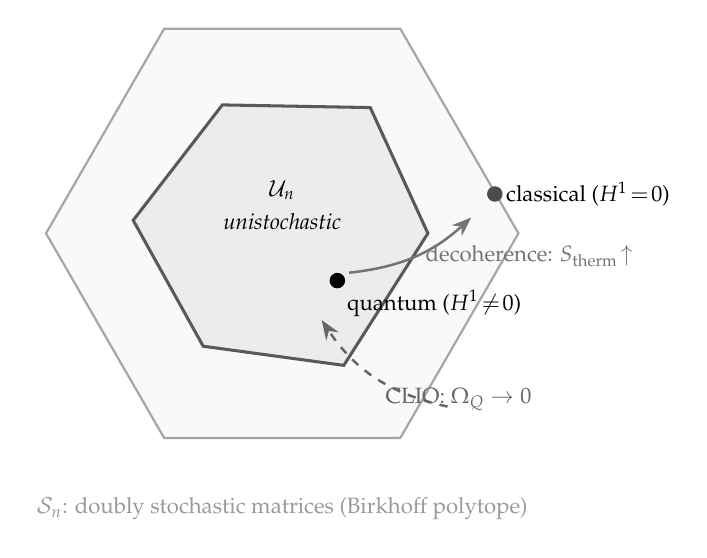
\begin{tikzpicture}[>=Stealth, font=\small]
  % Birkhoff polytope outline (hexagonal schematic)
  \draw[black!35, line width=0.8pt, fill=gray!5]
    (0:3.0) -- (60:3.0) -- (120:3.0) -- (180:3.0)
    -- (240:3.0) -- (300:3.0) -- cycle;
  \node[black!40, font=\footnotesize] at (0,-3.5)
    {$\mathcal{S}_n$: doubly stochastic matrices (Birkhoff polytope)};

  % Unistochastic subset (irregular inner region)
  \draw[black!65, line width=1.1pt, fill=gray!15]
    (0:1.85) -- (55:1.95) -- (115:1.80) -- (175:1.90)
    -- (235:1.75) -- (295:1.85) -- cycle;
  \node[font=\footnotesize] at (0,0.55) {$\mathcal{U}_n$};
  \node[font=\footnotesize\itshape] at (0,0.15) {unistochastic};

  % Classical boundary point
  \fill[black!70] (2.7,0.5) circle (2.8pt);
  \node[right, font=\footnotesize] at (2.72,0.5)
    {classical ($H^1\!=\!0$)};

  % Quantum interior point
  \fill[black] (0.7,-0.6) circle (2.8pt);
  \node[below right, font=\footnotesize] at (0.7,-0.6)
    {quantum ($H^1\!\neq\!0$)};

  % CLIO arrow toward U_n
  \draw[->, black!60, line width=0.9pt, dashed]
    (2.1,-2.2) to[bend left=22]
    node[below right, font=\footnotesize]
    {\CLIO: $\Omega_Q\to 0$}
    (0.5,-1.1);

  % Decoherence arrow exiting U_n
  \draw[->, black!55, line width=0.9pt]
    (0.85,-0.5) to[bend right=18]
    node[right, font=\footnotesize]
    {decoherence: $S_\mathrm{therm}\!\uparrow$}
    (2.4,0.2);
\end{tikzpicture}
\caption{Schematic slice of the Birkhoff polytope $\mathcal{S}_n$. The
unistochastic subset $\mathcal{U}_n$ (inner shaded region) is a strict
subset for $n\geq 3$. Quantum-admissible \RSVP\ projections lie in
$\mathcal{U}_n$; \CLIO\ obstruction minimization drives projected kernels
toward this region; decoherence (increasing $S_\mathrm{therm}$) drives them
out toward the classical boundary.}
\label{fig:unistochastic}
\end{figure}

\emph{Status: Ansatz.} Hilbert space is not introduced as an independent
ontology. It appears as the minimal phase-lift of an admissible stochastic
transition system. The scalar field $\Phi$ supplies amplitude structure, the
vector field $\mathbf{v}$ supplies directed transition phase, and the entropy
field $S_\mathrm{therm}$ measures information lost under projection.

\emph{Distinction from classical projection.} A merely stochastic coarse-graining
discards phase: $X(t)\mapsto P$. A quantum-admissible coarse-graining preserves
the possibility of phase reconstruction: $X(t)\mapsto U\mapsto P$ with
$P_{ij}=|U_{ij}|^2$.
\end{appansatz}

\begin{defn}[\claimD Born Amplitude from Scalar Capacity and Transport Phase]
Given a partition element $y_i\in\mathcal{Y}$, define the projected amplitude
\[
\psi_i
= \rho_i^{1/2}\,e^{i\theta_i},
\]
where the modulus is the entropy-weighted scalar capacity
\[
\rho_i
= \frac{\displaystyle\int_{\Pi^{-1}(y_i)} e^{-\beta S_\mathrm{therm}}\Phi^2\,d\mu}
         {\displaystyle\sum_j\int_{\Pi^{-1}(y_j)} e^{-\beta S_\mathrm{therm}}\Phi^2\,d\mu}
\]
and the phase is the transport holonomy
\[
\theta_i = \int_{\gamma_i}\mathbf{v}\cdot d\mathbf{x}
\]
along an admissible path $\gamma_i$ associated with $y_i$.
\end{defn}

Under this definition, observable probability is $p_i=|\psi_i|^2=\rho_i$: a
Born rule with entropy-weighted scalar capacity as the probability weight. The
magnitude is determined by scalar capacity filtered through thermodynamic
entropy, while the phase is transport holonomy. A unitary transition operator
$U_{ij}$ then evolves amplitudes by $\psi_j(t+\Delta t)=\sum_i U_{ji}\psi_i(t)$,
and observable transition probabilities are $P_{ij}=|U_{ij}|^2$.

\begin{appconj}[\claimC Born Rule as Entropy-Weighted Projection]
For any finite observable partition $\mathcal{Y}$ of the \RSVP\ field manifold,
if recursive transport preserves phase coherence and \CLIO\ obstruction is
minimized on $S_\mathrm{adm}$, then the induced probability measure on
$\mathcal{Y}$ is given by entropy-weighted scalar capacity:
\[
p_i
= \frac{\displaystyle\int_{\Pi^{-1}(y_i)} e^{-\beta S_\mathrm{therm}}\Phi^2\,d\mu}
         {\displaystyle\sum_j\int_{\Pi^{-1}(y_j)} e^{-\beta S_\mathrm{therm}}\Phi^2\,d\mu}.
\]
\emph{Status: Conjecture.} This is not a derivation of quantum mechanics. It
identifies the precise bridge that must be proved: phase-preserving \RSVP\
transport must induce unistochastic transition kernels whose projected weights
coincide with this Born measure.
\end{appconj}

\begin{appphen}[\claimP Quantum Measurement as Phase-Lift Failure]
Quantum measurement is interpreted as the loss of operational access to the
unitary phase lift of a projected \RSVP\ transition kernel. Before measurement,
the projected dynamics admits a unitary lift: $P=|U|^2$. Interaction with a
measuring environment increases local thermodynamic entropy $S_\mathrm{therm}
\mapsto S_\mathrm{therm}+\delta S$, suppressing phase-sensitive interference
by $\psi_i\mapsto e^{-\delta S_i/2}\psi_i$. As entropy grows, the unitary
lift is no longer operationally reconstructible and the effective transition
matrix approaches a classical stochastic matrix. Wavefunction collapse is not
introduced as a primitive dynamical event; it appears as the loss of
unistochastic structure under entropy increase and projection.

This interpretation has an analogue in the \CLIO\ reasoning framework
\cite{Cheng2025}: a coherent recursive branch remains stable when uncertainty
decreases and graph structure converges, while a failed branch loses
phase-like coherence between candidate trajectories and collapses to a
lower-resolution belief state.
\end{appphen}

\begin{defn}[\claimD Quantum Admissibility Obstruction]
Define the quantum admissibility obstruction functional
\[
\Omega_Q(P) = \mathrm{dist}(P,\mathcal{U}_n)^2,
\]
where the distance is measured in the Hilbert--Schmidt norm on $\mathcal{S}_n$.
The total enlarged obstruction functional is
\[
\Omega_\mathrm{total}
= \Omega_\mathrm{glue}
+ \Omega_\mathrm{geom}
+ \Omega_\mathrm{anom}
+ \Omega_Q.
\]
\end{defn}

\begin{appconj}[\claimC Quantum Admissibility Conjecture]
Low-obstruction \RSVP\ configurations project to transition kernels lying in
or arbitrarily close to the unistochastic subset $\mathcal{U}_n$. Classical
stochastic dynamics arise when entropy growth drives the projected kernel away
from $\mathcal{U}_n$ or destroys operational access to its phase lift. Under
this conjecture, quantum theory is the probability calculus of the
phase-liftable sector of recursive admissibility dynamics, and the hierarchy
\[
\begin{gathered}
\text{deterministic \RSVP\ transport} \\
\Downarrow \\
\text{projected stochastic transition} \\
\Downarrow \\
\text{unistochastic admissibility} \\
\Downarrow \\
\text{Hilbert-space quantum mechanics}
\end{gathered}
\]
constitutes the emergent reconstruction of quantum probability.
\end{appconj}

The geometry of $\mathcal{U}_n\subset\mathcal{S}_n$ is well-studied: the
unistochastic matrices form a proper subset of the Birkhoff polytope of doubly
stochastic matrices, and for $n\geq 3$ the inclusion is strict. The residual
mathematical obligation of this appendix is to characterize precisely when a
\RSVP\ projection $\Pi$ produces a transition matrix in $\mathcal{U}_n$,
and to determine whether \CLIO\ obstruction minimization on $\Omega_Q$ generically
favors unistochastic kernels. This would provide a constraint-first account of
why quantum probability appears in nature without being postulated as a
primitive structure.

% =================================================
\section{Temporal Architecture: Geometric Time and Admissibility Time}

The reconstruction program developed throughout this manuscript implicitly
inherits ordinary temporal evolution from the PDE framework of Section~2.
The \CLIO\ gradient flow parameter $t$ and the Lorentzian evolution parameter
of the underlying manifold $M$ are distinct objects that have not been
carefully separated. The present appendix distinguishes them and identifies
the structural tension this creates in the quantum reconstruction of
Appendix~J.

\begin{defn}[\claimD Geometric Time and Admissibility Time]
Let $t_\mathrm{geom}$ denote the temporal coordinate of the underlying
Lorentzian manifold $M$, governing the hyperbolic evolution of the \RSVP\
fields through the Euler--Lagrange system of Appendix~A. Let $t_\mathrm{adm}$
denote the parameter of the \CLIO\ gradient flow $dX/dt_\mathrm{adm}
=-\nabla\Omega(X)$ on admissibility space $\Field^{(s)}$. These are distinct:
$t_\mathrm{geom}$ is a coordinate on $M$ and determines causal structure,
while $t_\mathrm{adm}$ is a descent parameter on the space of field
configurations and determines obstruction reduction.
\end{defn}

The distinction matters for several reasons. First, the \CLIO\ flow need not
be compatible with Lorentzian causality: gradient descent on $\Omega$ can
move field configurations in ways that violate the causal order defined by
$g_{ij}$. This is not necessarily a defect of the framework; it may indicate
that admissibility closure is a trans-causal or background-independent
process that the underlying Lorentzian structure emerges from rather than
constrains. Second, the \TARTAN\ recursive projection operators
$\mathcal{R}_n:\Field_n\to\Field_{n+1}$ are defined in terms of spectral
scale rather than in terms of $t_\mathrm{geom}$, so the multiscale
renormalization architecture is naturally expressed in admissibility time.

\begin{ansatz}[\claimA Admissibility-First Temporal Architecture]
The physically observable Lorentzian time $t_\mathrm{geom}$ emerges as an
ordering relation on $t_\mathrm{adm}$-stable field configurations. That is,
physical causality is a property of the low-obstruction attractor structure
of admissibility space rather than a primitive property of the background
manifold.

\emph{Status: Ansatz.} This reverses the usual relationship between geometry
and dynamics. The conjecture that $t_\mathrm{geom}$ is recoverable from
$t_\mathrm{adm}$ ordering requires an explicit reconstruction theorem
analogous to the recovery of metric geometry from admissibility closure in
the metric-compatibility conjecture of Appendix~H.4.
\end{ansatz}

The temporal distinction also clarifies the quantum reconstruction of
Appendix~J. The unistochastic transition matrix $P_{ij}$ is defined for
transitions over a $t_\mathrm{geom}$ interval $\Delta t$, but the
phase-liftability condition is a property of the admissibility geometry of the
projected transition system. The Born amplitude
$\psi_i=\rho_i^{1/2}e^{i\theta_i}$ is built from scalar capacity and transport
holonomy, both of which depend on $t_\mathrm{adm}$-stable structures. Quantum
probability therefore measures properties of admissibility-time attractors
projected onto geometric-time transition intervals.

\begin{appconj}[\claimC Temporal Recovery Conjecture]
There exists a map $\Sigma: t_\mathrm{adm}\to t_\mathrm{geom}$ such that
the causal order on low-obstruction \RSVP\ configurations under $t_\mathrm{adm}$
descent maps bijectively to the partial causal order of the Lorentzian manifold
$(M,g)$. Under this map, geometric time is the observable shadow of
admissibility-descent ordering on the stable attractor manifold of the \CLIO\
flow.
\end{appconj}

% =================================================
\section{Sheaf-Theoretic Contextuality and Admissibility Obstructions}

The reconstruction program has employed sheaf theory throughout as the
natural language for local-to-global consistency. The present appendix
identifies a connection between the admissibility obstruction formalism
and sheaf-theoretic treatments of quantum contextuality in categorical
quantum foundations, as developed by Abramsky and Brandenburger \cite{AbramskyBrandenburger2011}.

In the Abramsky--Brandenburger framework, quantum contextuality arises when
a family of locally compatible probability distributions over measurement
outcomes fails to admit a global joint distribution. This is precisely the
obstruction to the existence of a global section of the observable sheaf:
local sections exist, but they cannot be assembled into a coherent global
section. The obstruction is measured by a cohomology class in $H^1$ of the
measurement cover, exactly analogous to the gluing obstructions of
Appendix~B.

\begin{appphen}[\claimP Contextuality as Admissibility Obstruction]
Quantum contextuality, in the Abramsky--Brandenburger sense, corresponds to a
nonvanishing first-order gluing obstruction $[\omega_1]\in H^1(M,\Sheaf_\mathrm{obs})$
of the observable sheaf $\Sheaf_\mathrm{obs}$ over the measurement context cover.
This is a special case of the \RSVP\ admissibility obstruction structure: the
measurement contexts play the role of local admissibility patches, and
contextuality corresponds to the failure of a global section of the projected
admissibility sheaf.

\emph{Status: Phenomenological Interpretation.} The identification of
$\Sheaf_\mathrm{obs}$ with a sub-sheaf of $\Sheaf_\RSVP$ under the observation
projection $\Pi$ is an interpretive proposal, not a derivation.
\end{appphen}

This connection has a direct implication for the Bell-locality tension
identified in the technical review. Bell-type nonlocality and Kochen--Specker
contextuality can both be expressed as obstructions to global sections of
observable sheaves. Within the \RSVP\ framework, these obstructions are
instances of the general obstruction classes $[\omega_k]\in H^k(M,\Sheaf_\RSVP)$.
The projection structure $\Pi$ determines which sub-sheaf is accessible to
local observers, and non-factorizability of joint measurement probabilities
corresponds to non-triviality of the projection-restricted cohomology.

The \CLIO\ operator, interpreted as a cohomological degree-lowering map, then
acts on contextuality obstructions in the same way it acts on gauge-gluing
obstructions: it attempts to reduce $H^1(M,\Sheaf_\mathrm{obs})$ toward zero.
Physical quantum systems live in the regime where contextuality obstructions
cannot be fully resolved --- they are stabilized by the topology of the
observable bundle --- while classical systems correspond to projections whose
observable sheaf admits a global section.

\begin{appconj}[\claimC Contextuality-Admissibility Correspondence]
The class of measurement scenarios exhibiting quantum contextuality corresponds
exactly to the class of \RSVP\ projections $\Pi$ for which the projected
admissibility sheaf $\Pi_\ast\Sheaf_\RSVP$ has nonvanishing first cohomology.
Classical probability arises from projections for which $H^1(M,\Pi_\ast\Sheaf_\RSVP)=0$,
and quantum probability from projections for which $H^1\neq 0$ but
$H^1(M,\Pi_\ast\Sheaf_\RSVP)$ is finitely generated and compatible with
unistochastic projection.
\end{appconj}

\newpage

% =================================================
% BIBLIOGRAPHY
% =================================================
\begin{thebibliography}{99}

\bibitem{Einstein1915}
Albert Einstein,
\textit{Die Feldgleichungen der Gravitation},
Sitzungsberichte der K\"{o}niglich Preussischen Akademie der Wissenschaften Berlin,
pp.~844--847, 1915.

\bibitem{Cartan1922}
\'{E}lie Cartan,
\textit{Sur une g\'{e}n\'{e}ralisation de la notion de courbure de Riemann et les espaces \`{a} torsion},
Comptes Rendus de l'Acad\'{e}mie des Sciences,
Vol.~174, pp.~593--595, 1922.

\bibitem{Weyl1918}
Hermann Weyl,
\textit{Gravitation und Elektrizit\"{a}t},
Sitzungsberichte der K\"{o}niglich Preussischen Akademie der Wissenschaften Berlin,
pp.~465--480, 1918.

\bibitem{YangMills1954}
Chen Ning Yang and Robert Mills,
\textit{Conservation of Isotopic Spin and Isotopic Gauge Invariance},
Physical Review, Vol.~96, No.~1, pp.~191--195, 1954.

\bibitem{Atiyah1978}
Michael Atiyah,
\textit{Geometry of Yang--Mills Fields},
Scuola Normale Superiore Pisa, 1978.

\bibitem{Nakahara2003}
Mikio Nakahara,
\textit{Geometry, Topology and Physics},
Second Edition, Institute of Physics Publishing, 2003.

\bibitem{BottTu1982}
Raoul Bott and Loring Tu,
\textit{Differential Forms in Algebraic Topology},
Springer, 1982.

\bibitem{MilnorStasheff1974}
John Milnor and James Stasheff,
\textit{Characteristic Classes},
Princeton University Press, 1974.

\bibitem{KobayashiNomizu1963}
Shoshichi Kobayashi and Katsumi Nomizu,
\textit{Foundations of Differential Geometry, Volume~I},
Interscience Publishers, 1963.

\bibitem{LawsonMichelsohn1989}
H.~Blaine Lawson and Marie-Louise Michelsohn,
\textit{Spin Geometry},
Princeton University Press, 1989.

\bibitem{EguchiGilkeyHanson1980}
Tohru Eguchi, Peter Gilkey, and Andrew Hanson,
\textit{Gravitation, Gauge Theories and Differential Geometry},
Physics Reports, Vol.~66, No.~6, pp.~213--393, 1980.

\bibitem{NashSen1983}
Charles Nash and Siddhartha Sen,
\textit{Topology and Geometry for Physicists},
Academic Press, 1983.

\bibitem{FrankGleiserThompson2024}
Adam Frank, Marcelo Gleiser, and Evan Thompson,
\textit{The Blind Spot: Why Science Cannot Ignore Human Experience},
MIT Press, 2024.

\bibitem{Simon1983}
Leon Simon,
\textit{Asymptotics for a Class of Nonlinear Evolution Equations, with Applications to Geometric Problems},
Annals of Mathematics, Vol.~118, No.~3, pp.~525--571, 1983.

\bibitem{Lojasiewicz1963}
Stanis\l{}aw Ło\-ja\-sie\-wicz,
\textit{Une propri\'{e}t\'{e} topologique des sous-ensembles analytiques r\'{e}els},
Les \'{E}quations aux D\'{e}riv\'{e}es Partielles,
\'{E}ditions du CNRS, pp.~87--89, 1963.


\bibitem{Hehl1995}
Friedrich Hehl, J.~D.~McCrea, Eckehard Mielke, and Yuval Ne'eman,
\textit{Metric-Affine Gauge Theory of Gravity: Field Equations, Noether Identities, World Spinors, and Breaking of Dilation Invariance},
Physics Reports, Vol.~258, pp.~1--171, 1995.

\bibitem{Hamilton1982b}
Richard Hamilton,
\textit{The Inverse Function Theorem of Nash and Moser},
Bulletin of the American Mathematical Society, Vol.~7, No.~1, pp.~65--222, 1982.

\bibitem{Hamilton1982}
Richard Hamilton,
\textit{Three-Manifolds with Positive Ricci Curvature},
Journal of Differential Geometry, Vol.~17, pp.~255--306, 1982.

\bibitem{Perelman2002}
Grigori Perelman,
\textit{The Entropy Formula for the Ricci Flow and its Geometric Applications},
arXiv:math/0211159, 2002.

\bibitem{Friston2010}
Karl Friston,
\textit{The Free-Energy Principle: A Unified Brain Theory?},
Nature Reviews Neuroscience, Vol.~11, pp.~127--138, 2010.

\bibitem{Cheng2025}
Newman Cheng, Gordon Broadbent, and William Chappell,
\textit{Cognitive Loop via In-Situ Optimization: Self-Adaptive Reasoning for Science},
arXiv:2508.02789, 2025.

\bibitem{Kadanoff1966}
Leo Kadanoff,
\textit{Scaling Laws for Ising Models Near $T_c$},
Physics Physique Fizika, Vol.~2, pp.~263--272, 1966.

\bibitem{Wilson1975}
Kenneth Wilson,
\textit{The Renormalization Group: Critical Phenomena and the Kondo Problem},
Reviews of Modern Physics, Vol.~47, pp.~773--840, 1975.

\bibitem{Connes1994}
Alain Connes,
\textit{Noncommutative Geometry},
Academic Press, 1994.

\bibitem{BaezMuniain1994}
John Baez and Javier P.~Muniain,
\textit{Gauge Fields, Knots and Gravity},
World Scientific, 1994.

\bibitem{Arnold1989}
Vladimir Arnold,
\textit{Mathematical Methods of Classical Mechanics},
Second Edition, Springer, 1989.

\bibitem{Besse1987}
Arthur Besse,
\textit{Einstein Manifolds},
Springer, 1987.

\bibitem{PenroseRindler1984}
Roger Penrose and Wolfgang Rindler,
\textit{Spinors and Space-Time, Volume~I},
Cambridge University Press, 1984.

\bibitem{Dirac1931}
Paul Dirac,
\textit{Quantised Singularities in the Electromagnetic Field},
Proceedings of the Royal Society A, Vol.~133, pp.~60--72, 1931.

\bibitem{AtiyahSinger1963}
Michael Atiyah and Isadore Singer,
\textit{The Index of Elliptic Operators on Compact Manifolds},
Bulletin of the American Mathematical Society, Vol.~69, pp.~422--433, 1963.

\bibitem{Witten1982}
Edward Witten,
\textit{An SU(2) Anomaly},
Physics Letters B, Vol.~117, pp.~324--328, 1982.

\bibitem{Brylinski1993}
Jean-Luc Brylinski,
\textit{Loop Spaces, Characteristic Classes and Geometric Quantization},
Birkh\"{a}user, 1993.

\bibitem{Gromov1999}
Mikhail Gromov,
\textit{Metric Structures for Riemannian and Non-Riemannian Spaces},
Birkh\"{a}user, 1999.

\bibitem{MacLane1998}
Saunders Mac~Lane,
\textit{Categories for the Working Mathematician},
Second Edition, Springer, 1998.

\bibitem{KashiwaraSchapira1990}
Masaki Kashiwara and Pierre Schapira,
\textit{Sheaves on Manifolds},
Springer, 1990.

\bibitem{Bredon1997}
Glen Bredon,
\textit{Sheaf Theory},
Second Edition, Springer, 1997.

\bibitem{Rosen1991}
Robert Rosen,
\textit{Life Itself: A Comprehensive Inquiry into the Nature, Origin, and Fabrication of Life},
Columbia University Press, 1991.

\bibitem{Varela1974}
Francisco Varela, Humberto Maturana, and Ricardo Uribe,
\textit{Autopoiesis: The Organization of Living Systems},
Biosystems, Vol.~5, pp.~187--196, 1974.

\bibitem{Kauffman1993}
Stuart Kauffman,
\textit{The Origins of Order: Self-Organization and Selection in Evolution},
Oxford University Press, 1993.

\bibitem{Jacobson1995}
Ted Jacobson,
\textit{Thermodynamics of Spacetime: The Einstein Equation of State},
Physical Review Letters, Vol.~75, pp.~1260--1263, 1995.

\bibitem{Verlinde2011}
Erik Verlinde,
\textit{On the Origin of Gravity and the Laws of Newton},
Journal of High Energy Physics, Vol.~2011, No.~29, 2011.


\bibitem{AbramskyBrandenburger2011}
Samson Abramsky and Adam Brandenburger,
\textit{The Sheaf-Theoretic Structure of Non-Locality and Contextuality},
New Journal of Physics, Vol.~13, 113036, 2011.

\bibitem{Gilkey1995}
Peter Gilkey,
\textit{Invariance Theory, the Heat Equation, and the Atiyah--Singer Index Theorem},
Second Edition, CRC Press, 1995.

\end{thebibliography}

\end{document}